% =======================
% Chapter: Appendix
%
% Author: Daniel Wehner
%

% Probing Task Setup
% -----------------------------------------------------------------------------------------------------------------------------------------------------
\section{Probing Task Setup}
\label{sec:appendix_probing_task_setup}

% Table: 30 chosen nouns for each language
\begin{table}[h]
	\centering
	\renewcommand{\arraystretch}{0.90}
	\scalebox{0.90}{
	\begin{tabularx}{\textwidth}{| X | X | X | X | X |}
		\hline
		\rowcolor{tud9c!50}
		\textbf{EN}	&
		\textbf{DE} 	&
		\textbf{RU} 	&
		\textbf{TR}	&
		\textbf{KA} 	\\
		\hline\hline
		project		& Insel			& \foreignlanguage{russian}{миллионов}		& vergi			&
					\multirow{30}{*}{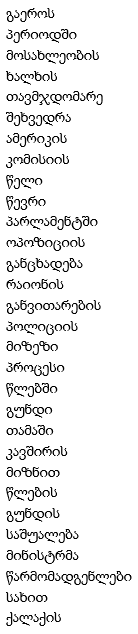
\includegraphics[scale=0.665]{images/wc_ka_list}}\\
		horse		& Norden		& \foreignlanguage{russian}{информации}		& yüzde			& \\
		dinner		& Bevölkerung	& \foreignlanguage{russian}{территории}		& karşılık		& \\
		countries	& Partei			& \foreignlanguage{russian}{рынке}			& Devlet			& \\
		restaurant	& Arten			& \foreignlanguage{russian}{программы}		& sırasında		& \\
		back		& Stunden		& \foreignlanguage{russian}{уровень}			& makine		& \\
		women		& Zahl			& \foreignlanguage{russian}{начала}			& içeriye			& \\
		Percentage	& Mannschaft		& \foreignlanguage{russian}{производства}		& okula			& \\
		moment		& Tochter		& \foreignlanguage{russian}{степени}			& mektup		& \\
		changes		& Provinz		& \foreignlanguage{russian}{период}			& haber			& \\
		minutes		& Laden			& \foreignlanguage{russian}{ходе}				& sahibi			& \\
		members	& Betrieb		& \foreignlanguage{russian}{средства}			& Kuzey			& \\
		security		& Beginn		& \foreignlanguage{russian}{основе}			& cevap			& \\
		reason		& Bedeutung		& \foreignlanguage{russian}{граждан}			& şirketi			& \\
		email		& Süden			& \foreignlanguage{russian}{отношения}		& yüzyılda		& \\
		language	& Wochen		& \foreignlanguage{russian}{движения}		& yüzünden		& \\
		peace		& Westen		& \foreignlanguage{russian}{данным}			& dönemde		& \\
		position		& Ergebnis		& \foreignlanguage{russian}{большинство}		& durumunda	& \\
		girl			& Minuten		& \foreignlanguage{russian}{безопасности}		& yola			& \\
		PivotTable	& Dorf			& \foreignlanguage{russian}{участие}			& öğrenci		& \\
		level		& Länge			& \foreignlanguage{russian}{взгляд}			& çocuğun		& \\
		city			& Vertrag		& \foreignlanguage{russian}{культуры}			& sorun			& \\
		agreement	& Jahrhundert	& \foreignlanguage{russian}{группы}			& oğlum			& \\
		table		& Ortsteil		& \foreignlanguage{russian}{директор}			& seçim			& \\
		front		& Landkreis		& \foreignlanguage{russian}{проект}			& isim			& \\
		control		& Hilfe			& \foreignlanguage{russian}{армии}			& doğum		& \\
		others		& Verein			& \foreignlanguage{russian}{положение}		& ilişki			& \\
		thanks		& Hälfte			& \foreignlanguage{russian}{действия}			& masanın		& \\
		attention		& Verbindung	& \foreignlanguage{russian}{целом}			& gözleri			& \\
		hotel		& Zeitpunkt		& \foreignlanguage{russian}{смысле}			& ayında			& \\
		\hline
	\end{tabularx}}
	\caption[List of the 30 chosen mid-frequency nouns for each language (\caps{WC} task)]
		{List of the 30 chosen mid-frequency nouns for each language (\caps{WC} task). The table entries are sorted by frequencies.}
	\label{tab:wc_words}
\end{table}

\newpage

% Table: Chosen verbs for each language
\begin{table}[h]
	\centering
	\renewcommand{\arraystretch}{0.90}
	\scalebox{0.90}{
	\begin{tabularx}{\textwidth}{| X | X | X | X | X |}
		\hline
		\rowcolor{tud9c!50}
		\textbf{EN}	&
		\textbf{DE} 	&
		\textbf{RU} 	&
		\textbf{TR}	&
		\textbf{KA} 	\\
		\hline\hline
		know 		&	sein			&	\foreignlanguage{russian}{знать}		&	yapmak		&
			\multirow{38}{*}{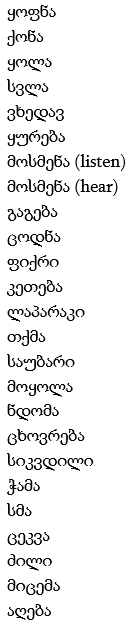
\includegraphics[scale=0.72]{images/sv_agree_ka_list}}	\\
		speak		&	tun			&	\foreignlanguage{russian}{жить}		&	gitmek		& 	\\
		think		&	gehen		&	\foreignlanguage{russian}{любитъ}	&	gelmek		& 	\\
		understand	&	machen		&	\foreignlanguage{russian}{работать}	&	almak		& 	\\
		remember	&	wissen		&	\foreignlanguage{russian}{ждать}		&	istemek		& 	\\
		eat			&	leben		&	\foreignlanguage{russian}{говорить}	&	çalışmak		& 	\\
		happen		&	arbeiten		&	\foreignlanguage{russian}{думать}		&	bilmek		& 	\\
		get			&	warten		&	\foreignlanguage{russian}{понимать}	&	konuşmak	& 	\\
		come		&	sprechen		&	\foreignlanguage{russian}{мочь}		&	okumak		& 	\\
		avoid		&	denken		&	\foreignlanguage{russian}{хотеть}		&	sevmek		& 	\\
		pretend		&	verstehen	&	\foreignlanguage{russian}{делать}		&	demek		& 	\\
		mitigate		&	wollen		&	\foreignlanguage{russian}{брать}		&	düşünmek	& 	\\
		pray			&	nehmen		&	\foreignlanguage{russian}{давать}		&	yemek		& 	\\
		forgive		&	geben		&	\foreignlanguage{russian}{помнить}	&	içmek		& 	\\
					&	sagen		&										&	başlamak	& 	\\
					&	fragen		&										&	olmak		& 	\\
					&	trinken		&										&	söylemek	& 	\\
					&	essen		&										&	yatmak		& 	\\
					&	passieren	&										&	oturmak		& 	\\
					&	mögen		&										&	sormak		& 	\\
					&	fliegen		&										&	inanmak		& 	\\
					&	haben		&										&	açıklamak	& 	\\
					&				&										&	açmak		&	\\
					&				&										&	affetmek		&	\\
					&				&										&	almak		&	\\
					&				&										&	anlamak		&	\\
					&				&										&	aramak		&	\\
					&				&										&	ağlamak		&	\\
					&				&										&	abartmak	&	\\
					&				&										&	beğenmek	&	\\
					&				&										&	beklemek	&	\\
					&				&										&	atlamak		&	\\
					&				&										&	atmak		&	\\
					&				&										&	azaltmak		&	\\
					&				&										&	korkmak		&	\\
					&				&										&	koşmak		&	\\
					&				&										&	kullanmak	&	\\	
					& 				&	 									&	önermek		&	\\				
		\hline
	\end{tabularx}}
	\caption[List of the chosen verbs for each language (\caps{SVAgree} task)]
		{List of the chosen verbs for each language (\caps{SVAgree} task).}
	\label{tab:sv_agree_words}
\end{table}

\vfill
\hrule
\textbf{Remarks concerning the tables in appendix \vref{sec:appendix_probing} and \vref{sec:appendix_downstream}:} \\
The following tables list the results on probing tasks and downstream tasks in detail. Next to the test scores, the tables furthermore contain the relative rankings of the embeddings per task. These rankings can be found in the columns labeled with `R'. In order to facilitate a quick overview, the top-three performances were highlighted: A \textcolor{gold}{golden} cell background indicates rank 1, \textcolor{silver}{silver} color rank 2, and finally, a \textcolor{bronze}{bronze} color denotes rank 3. The results were produced without hyper-parameter optimization.

\newpage

% Detailed Probing Task Results
% -----------------------------------------------------------------------------------------------------------------------------------------------------
\section{Detailed Probing Task Results}
\label{sec:appendix_probing}

% Results measured by F1 Score
% -----------------------------------------------------------------------------------------------------------------------------------------------------
\subsection{Results measured by F1 Score}

\begin{table}[H]
	\centering
	\renewcommand{\arraystretch}{1.36}
	\begin{adjustbox}{angle=90}
	\scalebox{0.8}{
	\begin{tabularx}{1.1\textheight}{
		| l ? Y | c | Y | c ? Y | c | Y | c | Y | c | Y | c | Y | c ? Y | c | Y | c |
	}
	\hline
	\multicolumn{19}{| c |}{
		\cellcolor{tud9c}\textcolor{white}{
			\textbf{Language: English (F1)}}} 					\\
	\hline

	\rowcolor{tud9c!85}
	\cellcolor{tud9c!85}										&
	\multicolumn{4}{ c ?}{\textbf{Surface Tasks}} 				& 
		\multicolumn{10}{ c ?}{\textbf{Syntactic Tasks}}		&
		\multicolumn{4}{c |}{\textbf{Semantic Tasks}}			\\

	\cellcolor{tud9c!85}										& 
		\multicolumn{2}{ c |}{
			\cellcolor{tud9c!70}\textbf{\caps{SentLen}}} 		&
		\multicolumn{2}{ c ?}{
			\cellcolor{tud9c!70}\textbf{\caps{WC}}} 			&
		\multicolumn{2}{ c |}{
			\cellcolor{tud9c!70}\textbf{\caps{BiShift}}}			&
		\multicolumn{2}{ c |}{
			\cellcolor{tud9c!70}\textbf{\caps{SVAgree}}} 		&
		\multicolumn{2}{ c |}{
			\cellcolor{tud9c!70}\textbf{\caps{SVDist}}} 			&
		\multicolumn{2}{ c |}{
			\cellcolor{tud9c!70}\textbf{\caps{Voice}}}			&
		\multicolumn{2}{ c ?}{
			\cellcolor{tud9c!70}\textbf{\caps{WO}}}			&
		\multicolumn{2}{ c |}{
			\cellcolor{tud9c!70}\textbf{\caps{EOS}}} 			&
		\multicolumn{2}{ c |}{
			\cellcolor{tud9c!70}\textbf{\caps{SubjNum}}}		\\

	\rowcolor{tud9c!55}
	\multirow{-3}{*}{\cellcolor{tud9c!85}\textbf{Embedding}}	&
		\textbf{F1} & \textbf{R} & \textbf{F1} & \textbf{R} & \textbf{F1} & \textbf{R} &
	   	\textbf{F1} & \textbf{R} & \textbf{F1} & \textbf{R} & \textbf{F1} & \textbf{R} &
	   	\textbf{F1} & \textbf{R} & \textbf{F1} & \textbf{R} & \textbf{F1} & \textbf{R} \\
	\hline\hline
	\multicolumn{19}{| l |}{\cellcolor{tud9c!30}\textbf{Size of the data set}} \\ \hline
	\# instances &
                10,000 	& - &
                10,000 	& - &
                10,000 	& - &
                10,000 	& - &
                10,000 	& - &
                9,999 		& - &
                10,000 	& - &
		   10,000 	& - &
                9,448 		& - \\   
	\hline\hline 
	\multicolumn{19}{| l |}{\cellcolor{tud9c!30}\textbf{Majority class (baseline)}} \\ \hline
	\rowcolor{lightgray!30}
	Majority &
                17.9 & - &
                13.3 & - &
                50.2 & - &
                51.1 & - &
                47.5 & - &
                61.0 & - &
                33.4 & - &
		   21.7 & - &
                75.7 & - \\
	\hline\hline   
	\multicolumn{19}{| l |}{\cellcolor{tud9c!30}\textbf{Random embeddings (baseline)}} \\ \hline
	\rowcolor{lightgray!30}
	BOREP &
                00.438 & 10 &
                00.551 & 18 &
                00.488 & 18 &
                00.737 & 18 &
                00.279 & 10 &
                00.776 & 10 &
                00.188 & 15 &
                00.213 & 10 &
                00.844 & 7 \\
        \hline
	 \rowcolor{lightgray!30}
        Random BiLSTM &
                00.549 & 7 &
                00.462 & 20 &
                00.510 & 6 &
                00.819 & 12 &
                00.323 & 5 &
                \cellcolor{bronze}{00.833} & \cellcolor{bronze}{3} &
                00.598 & 4 &
                \cellcolor{bronze}{00.246} & \cellcolor{bronze}{3} &
                \cellcolor{silver}{00.879} & \cellcolor{silver}{2} \\
	\hline\hline
	\multicolumn{19}{| l |}{\cellcolor{tud9c!30}\textbf{Average embeddings (\textit{FastText})}} \\ \hline
	Vanilla average &
                00.240 & 17 &
                00.581 & 17 &
                00.485 & 20 &
                00.775 & 16 &
                00.265 & 13 &
                00.798 & 7 &
                00.201 & 11 &
                00.150 & 19 &
                00.855 & 5 \\
        \hline
        p-Means &
                00.553 & 5 &
                00.657 & 13 &
                00.491 & 15 &
                00.804 & 14 &
                00.309 & 6 &
                00.807 & 6 &
                00.173 & 19 &
                00.231 & 6 &
                00.850 & 6 \\
        \hline
        SIF &
                00.217 & 19 &
                00.634 & 14 &
                00.471 & 21 &
                00.808 & 13 &
                00.256 & 15 &
                00.756 & 15 &
                00.208 & 10 &
                00.144 & 20 &
                00.835 & 8 \\
        \hline
        GEM &
                00.301 & 13 &
                00.778 & 10 &
                00.496 & 11 &
                00.776 & 15 &
                00.300 & 8 &
                00.718 & 19 &
                00.068 & 22 &
                00.206 & 12 &
                00.797 & 10 \\
        \hline
        hier. pooling &
                00.454 & 9 &
                00.354 & 22 &
                00.501 & 9 &
                00.660 & 21 &
                00.271 & 12 &
                00.779 & 8 &
                00.363 & 8 &
                00.232 & 5 &
                00.817 & 9 \\
	\hline\hline
	\multicolumn{19}{| l |}{\cellcolor{tud9c!30}\textbf{Average embeddings (\textit{word2vec})}} \\ \hline
	Vanilla average &
                00.243 & 16 &
                00.803 & 7 &
                00.497 & 10 &
                00.892 & 6 &
                00.255 & 16 &
                00.760 & 13 &
                00.187 & 16 &
                00.172 & 16 &
                00.659 & 17 \\
        \hline
        p-Means &
                00.503 & 8 &
                00.822 & 5 &
                00.502 & 8 &
                \cellcolor{gold}{00.939} & \cellcolor{gold}{1} &
                00.295 & 9 &
                00.764 & 12 &
                00.183 & 18 &
                00.236 & 4 &
                00.656 & 18 \\
        \hline
        SIF &
                00.215 & 20 &
                00.809 & 6 &
                00.506 & 7 &
                00.889 & 8 &
                00.248 & 18 &
                00.741 & 17 &
                00.191 & 14 &
                00.158 & 18 &
                00.619 & 21 \\
        \hline
        GEM &
                00.256 & 14 &
                00.597 & 16 &
                00.494 & 13 &
                00.710 & 20 &
                00.241 & 22 &
                00.684 & 21 &
                00.111 & 21 &
                00.179 & 15 &
                00.573 & 22 \\
        \hline
        hier. pooling &
                00.355 & 12 &
                00.695 & 12 &
                00.493 & 14 &
                00.841 & 10 &
                00.253 & 17 &
                00.724 & 18 &
                00.233 & 9 &
                00.224 & 8 &
                00.633 & 20 \\
	\hline\hline
	\multicolumn{19}{| l |}{\cellcolor{tud9c!30}\textbf{Average embeddings (\textit{Attract-Repel})}} \\ \hline
	Vanilla average &
                00.183 & 21 &
                00.622 & 15 &
                00.491 & 15 &
                00.890 & 7 &
                00.247 & 19 &
                00.753 & 16 &
                00.198 & 13 &
                00.141 & 21 &
                00.738 & 14 \\
        \hline
        p-Means &
                00.585 & 4 &
                \cellcolor{gold}{00.946} & \cellcolor{gold}{1} &
                00.464 & 22 &
                \cellcolor{silver}{00.936} & \cellcolor{silver}{2} &
                00.279 & 10 &
                00.818 & 4 &
                00.186 & 17 &
                00.210 & 11 &
                00.761 & 11 \\
        \hline
        SIF &
                00.162 & 22 &
                00.737 & 11 &
                00.488 & 18 &
                00.903 & 5 &
                00.243 & 21 &
                00.699 & 20 &
                00.200 & 12 &
                00.130 & 22 &
                00.685 & 16 \\
        \hline
        GEM &
                00.230 & 18 &
                00.803 & 7 &
                00.491 & 15 &
                00.743 & 17 &
                00.259 & 14 &
                00.650 & 22 &
                00.148 & 20 &
                00.167 & 17 &
                00.640 & 19 \\
        \hline
        hier. pooling &
                00.419 & 11 &
                00.406 & 21 &
                00.496 & 11 &
                00.835 & 11 &
                00.245 & 20 &
                00.770 & 11 &
                00.370 & 7 &
                00.193 & 13 &
                00.700 & 15 \\
	\hline\hline
	\multicolumn{19}{| l |}{\cellcolor{tud9c!30}\textbf{Trained embeddings}} \\ \hline
	InferSent &
                \cellcolor{bronze}{00.600} & \cellcolor{bronze}{3} &
                \cellcolor{silver}{00.919} & \cellcolor{silver}{2} &
                00.536 & 4 &
                \cellcolor{bronze}{00.912} & \cellcolor{bronze}{3} &
                \cellcolor{silver}{00.414} & \cellcolor{silver}{2} &
                \cellcolor{silver}{00.868} & \cellcolor{silver}{2} &
                \cellcolor{bronze}{00.760} & \cellcolor{bronze}{3} &
                00.230 & 7 &
                \cellcolor{silver}{00.879} & \cellcolor{silver}{2} \\
        \hline
        Quick-Thought &
                \cellcolor{silver}{00.649} & \cellcolor{silver}{2} &
                \cellcolor{bronze}{00.848} & \cellcolor{bronze}{3} &
                \cellcolor{bronze}{00.544} & \cellcolor{bronze}{3} &
                00.887 & 9 &
                \cellcolor{bronze}{00.410} & \cellcolor{bronze}{3} &
                00.811 & 5 &
                \cellcolor{silver}{00.802} & \cellcolor{silver}{2} &
                00.221 & 9 &
                00.758 & 13 \\
        \hline
        sent2vec &
                00.254 & 15 &
                00.786 & 9 &
                00.534 & 5 &
                00.910 & 4 &
                00.301 & 7 &
                00.779 & 8 &
                00.381 & 6 &
                00.191 & 14 &
                00.759 & 12 \\
        \hline
        BERT &
                00.551 & 6 &
                00.531 & 19 &
                \cellcolor{gold}{00.641} & \cellcolor{gold}{1} &
                00.718 & 19 &
                00.406 & 4 &
                00.760 & 13 &
                00.573 & 5 &
                \cellcolor{silver}{00.282} & \cellcolor{silver}{2} &
                00.858 & 4 \\
        \hline
        LASER &
                \cellcolor{gold}{00.697} & \cellcolor{gold}{1} &
                00.832 & 4 &
                \cellcolor{silver}{00.600} & \cellcolor{silver}{2} &
                00.572 & 22 &
                \cellcolor{gold}{00.521} & \cellcolor{gold}{1} &
                \cellcolor{gold}{00.904} & \cellcolor{gold}{1} &
                \cellcolor{gold}{00.846} & \cellcolor{gold}{1} &
                \cellcolor{gold}{00.319} & \cellcolor{gold}{1} &
                \cellcolor{gold}{00.899} & \cellcolor{gold}{1} \\
	\hline
	\end{tabularx}}
	\end{adjustbox}
	\caption[Probing task results for the English language (F1 scores)]{Probing task results for the English language (F1 scores).}
	\label{tab:results_probing_tasks_en}
\end{table}	
\begin{table}[H]
	\centering
	\renewcommand{\arraystretch}{1.36}
	\begin{adjustbox}{angle=90}
	\scalebox{0.8}{
	\begin{tabularx}{1.2\textheight}{
		| l ? Y | c | Y | c ? Y | c | Y | c | Y | c | Y | c | Y | c ? Y | c | Y | c |
	}
	\hline
	\multicolumn{19}{| c |}{
		\cellcolor{tud9c}\textcolor{white}{
			\textbf{Language: German (F1)}}} 					\\
	\hline

	\rowcolor{tud9c!85}
	\cellcolor{tud9c!85}										&
	\multicolumn{4}{ c ?}{\textbf{Surface Tasks}} 				& 
		\multicolumn{10}{ c ?}{\textbf{Syntactic Tasks}}		&
		\multicolumn{4}{c |}{\textbf{Semantic Tasks}}			\\

	\cellcolor{tud9c!85}										& 
		\multicolumn{2}{ c |}{
			\cellcolor{tud9c!70}\textbf{\caps{SentLen}}} 		&
		\multicolumn{2}{ c ?}{
			\cellcolor{tud9c!70}\textbf{\caps{WC}}} 			&
		\multicolumn{2}{ c |}{
			\cellcolor{tud9c!70}\textbf{\caps{BiShift}}}			&
		\multicolumn{2}{ c |}{
			\cellcolor{tud9c!70}\textbf{\caps{SVAgree}}}		&
		\multicolumn{2}{ c |}{
			\cellcolor{tud9c!70}\textbf{\caps{SVDist}}} 			&
		\multicolumn{2}{ c |}{
			\cellcolor{tud9c!70}\textbf{\caps{Voice}}}			&
		\multicolumn{2}{ c ?}{
			\cellcolor{tud9c!70}\textbf{\caps{WO}}}			&
		\multicolumn{2}{ c |}{
			\cellcolor{tud9c!70}\textbf{\caps{EOS}}} 			&
		\multicolumn{2}{ c |}{
			\cellcolor{tud9c!70}\textbf{\caps{SubjNum}}}		\\

	\rowcolor{tud9c!55}
	\multirow{-3}{*}{\cellcolor{tud9c!85}\textbf{Embedding}}	&
		\textbf{F1} & \textbf{R} & \textbf{F1} & \textbf{R} & \textbf{F1} & \textbf{R} &
		\textbf{F1} & \textbf{R} & \textbf{F1} & \textbf{R} & \textbf{F1} & \textbf{R} &
		\textbf{F1} & \textbf{R} & \textbf{F1} & \textbf{R} & \textbf{F1} & \textbf{R} \\
	\hline\hline
	\multicolumn{19}{| l |}{\cellcolor{tud9c!30}\textbf{Size of the data set}} \\ \hline
	\# instances &
                10,000 	& - &
                10,000 	& - &
                10,000 	& - &
                10,000 	& - &
                10,000 	& - &
                9,999	 	& - &
		   10,000 	& - &
                10,000 	& - &
                9,999	 	& - \\   
	\hline\hline 
	\multicolumn{19}{| l |}{\cellcolor{tud9c!30}\textbf{Majority class (baseline)}} \\ \hline
	\rowcolor{lightgray!30}
	Majority &
                19.9 & - &
                14.8 & - &
                50.2 & - &
                50.7 & - &
                43.6 & - &
                50.0 & - &
                33.4 & - &
		   19.3 & - &
                50.0 & - \\
	\hline\hline   
	\multicolumn{19}{| l |}{\cellcolor{tud9c!30}\textbf{Random embeddings (baseline)}} \\ \hline
	\rowcolor{lightgray!30}
	BOREP &
                00.402 & 10 &
                00.668 & 7 &
                00.482 & 22 &
                \cellcolor{silver}{00.846} & \cellcolor{silver}{2} &
                00.327 & 10 &
                00.790 & 17 &
                00.173 & 22 &
                00.205 & 11 &
                00.858 & 15 \\
        \hline
        \rowcolor{lightgray!30}
        Random BiLSTM &
                00.508 & 4 &
                00.577 & 8 &
                00.490 & 16 &
                \cellcolor{gold}{00.847} & \cellcolor{gold}{1} &
                00.399 & 4 &
                00.864 & 4 &
                \cellcolor{silver}{00.735} & \cellcolor{silver}{2} &
                00.229 & 8 &
                00.895 & 7 \\
	\hline\hline
	\multicolumn{19}{| l |}{\cellcolor{tud9c!30}\textbf{Average embeddings (\textit{FastText})}} \\ \hline
	Vanilla average &
                00.195 & 15 &
                00.695 & 6 &
                00.489 & 18 &
                00.822 & 10 &
                00.318 & 14 &
                00.832 & 12 &
                00.215 & 16 &
                00.172 & 15 &
                \cellcolor{bronze}{00.903} & \cellcolor{bronze}{3} \\
        \hline
        p-Means &
                00.492 & 6 &
                00.745 & 4 &
                00.489 & 18 &
                00.837 & 5 &
                00.336 & 9 &
                00.856 & 7 &
                00.199 & 20 &
                00.232 & 6 &
                00.890 & 9 \\
        \hline
        SIF &
                00.164 & 18 &
                00.737 & 5 &
                00.500 & 10 &
                00.813 & 12 &
                00.293 & 17 &
                00.793 & 15 &
                00.216 & 14 &
                00.153 & 19 &
                00.898 & 5 \\
        \hline
        GEM &
                00.249 & 14 &
                \cellcolor{bronze}{00.816} & \cellcolor{bronze}{3} &
                00.512 & 5 &
                00.830 & 7 &
                00.325 & 11 &
                00.854 & 8 &
                00.222 & 12 &
                00.198 & 12 &
                00.889 & 10 \\
        \hline
        hier. pooling &
                00.433 & 9 &
                00.524 & 10 &
                00.492 & 13 &
                00.794 & 15 &
                00.322 & 13 &
                00.762 & 20 &
                00.451 & 6 &
                00.217 & 9 &
                00.833 & 16 \\
	\hline\hline
	\multicolumn{19}{| l |}{\cellcolor{tud9c!30}\textbf{Average embeddings (\textit{word2vec})}} \\ \hline
	Vanilla average &
                00.170 & 17 &
                00.296 & 13 &
                00.491 & 15 &
                00.826 & 8 &
                00.337 & 8 &
                00.860 & 5 &
                00.226 & 11 &
                00.154 & 18 &
                00.891 & 8 \\
        \hline
        p-Means &
                00.482 & 7 &
                00.255 & 15 &
                00.500 & 10 &
                00.818 & 11 &
                00.325 & 11 &
                00.858 & 6 &
                00.174 & 21 &
                00.231 & 7 &
                00.883 & 11 \\
        \hline
        SIF &
                00.143 & 21 &
                00.284 & 14 &
                00.504 & 7 &
                00.800 & 14 &
                00.312 & 15 &
                00.839 & 10 &
                00.220 & 13 &
                00.141 & 21 &
                00.880 & 13 \\
        \hline
        GEM &
                00.185 & 16 &
                00.157 & 19 &
                00.503 & 8 &
                00.640 & 21 &
                00.254 & 20 &
                00.664 & 22 &
                00.205 & 19 &
                00.162 & 16 &
                00.650 & 22 \\
        \hline
        hier. pooling &
                00.280 & 12 &
                00.242 & 16 &
                00.492 & 13 &
                00.790 & 17 &
                00.311 & 16 &
                00.819 & 13 &
                00.249 & 10 &
                00.192 & 14 &
                00.865 & 14 \\
	\hline\hline
	\multicolumn{19}{| l |}{\cellcolor{tud9c!30}\textbf{Average embeddings (\textit{Attract-Repel})}} \\ \hline
	Vanilla average &
                00.156 & 20 &
                00.154 & 20 &
                00.495 & 12 &
                00.808 & 13 &
                00.261 & 19 &
                00.798 & 14 &
                00.216 & 14 &
                00.149 & 20 &
                00.808 & 18 \\
        \hline
        p-Means &
                00.500 & 5 &
                00.238 & 17 &
                00.487 & 20 &
                00.840 & 4 &
                00.339 & 7 &
                \cellcolor{gold}{00.877} & \cellcolor{gold}{1} &
                00.211 & 17 &
                00.237 & 5 &
                00.828 & 17 \\
        \hline
        SIF &
                00.128 & 22 &
                00.130 & 21 &
                00.486 & 21 &
                00.793 & 16 &
                00.224 & 22 &
                00.764 & 19 &
                00.209 & 18 &
                00.123 & 22 &
                00.791 & 19 \\
        \hline
        GEM &
                00.162 & 19 &
                00.185 & 18 &
                00.502 & 9 &
                00.663 & 20 &
                00.239 & 21 &
                00.744 & 21 &
                00.250 & 9 &
                00.161 & 17 &
                00.741 & 21 \\
        \hline
        hier. pooling &
                00.342 & 11 &
                00.128 & 22 &
                00.490 & 16 &
                00.774 & 18 &
                00.270 & 18 &
                00.781 & 18 &
                00.324 & 8 &
                00.211 & 10 &
                00.759 & 20 \\
	\hline\hline
	\multicolumn{19}{| l |}{\cellcolor{tud9c!30}\textbf{Trained embeddings}} \\ \hline
	InferSent &
                \cellcolor{silver}{00.557} & \cellcolor{silver}{2} &
                00.449 & 11 &
                00.505 & 6 &
                00.834 & 6 &
                00.367 & 6 &
                00.838 & 11 &
                \cellcolor{bronze}{00.713} & \cellcolor{bronze}{3} &
                00.242 & 4 &
                00.882 & 12 \\
        \hline
        Quick-Thought &
                \cellcolor{bronze}{00.520} & \cellcolor{bronze}{3} &
                00.346 & 12 &
                \cellcolor{bronze}{00.575} & \cellcolor{bronze}{3} &
                00.825 & 9 &
                \cellcolor{gold}{00.456} & \cellcolor{gold}{1} &
                \cellcolor{bronze}{00.868} & \cellcolor{bronze}{3} &
                00.490 & 5 &
                \cellcolor{silver}{00.269} & \cellcolor{silver}{2} &
                00.901 & 4 \\
        \hline
        sent2vec &
                00.271 & 13 &
                \cellcolor{gold}{00.968} & \cellcolor{gold}{1} &
                00.521 & 4 &
                \cellcolor{bronze}{00.845} & \cellcolor{bronze}{3} &
                00.370 & 5 &
                \cellcolor{silver}{00.874} & \cellcolor{silver}{2} &
                00.429 & 7 &
                00.197 & 13 &
                \cellcolor{gold}{00.906} & \cellcolor{gold}{1} \\
        \hline
        BERT &
                00.467 & 8 &
                00.577 & 8 &
                \cellcolor{gold}{00.636} & \cellcolor{gold}{1} &
                00.771 & 19 &
                \cellcolor{bronze}{00.404} & \cellcolor{bronze}{3} &
                00.793 & 15 &
                00.584 & 4 &
                \cellcolor{silver}{00.269} & \cellcolor{silver}{2} &
                00.896 & 6 \\
        \hline
        LASER &
                \cellcolor{gold}{00.608} & \cellcolor{gold}{1} &
                \cellcolor{silver}{00.861} & \cellcolor{silver}{2} &
                \cellcolor{silver}{00.606} & \cellcolor{silver}{2} &
                00.639 & 22 &
                \cellcolor{silver}{00.448} & \cellcolor{silver}{2} &
                00.854 & 8 &
                \cellcolor{gold}{00.821} & \cellcolor{gold}{1} &
                \cellcolor{gold}{00.307} & \cellcolor{gold}{1} &
                \cellcolor{silver}{00.905} & \cellcolor{silver}{2} \\
	\hline
	\end{tabularx}}
	\end{adjustbox}
	\caption[Probing task results for the German language (F1 scores)]{Probing task results for the German language (F1 scores).}
	\label{tab:results_probing_tasks_de}
\end{table}	
\begin{table}[H]
	\centering
	\renewcommand{\arraystretch}{1.36}
	\begin{adjustbox}{angle=90}
	\scalebox{0.8}{
	\begin{tabularx}{1.2\textheight}{
		| l ? Y | c | Y | c ? Y | c | Y | c | Y | c | Y | c | Y | c ? Y | c | Y | c |
	}
	\hline
	\multicolumn{19}{| c |}{
		\cellcolor{tud9c}\textcolor{white}{
			\textbf{Language: Russian (F1)}}} 					\\
	\hline

	\rowcolor{tud9c!85}
	\cellcolor{tud9c!85}										&
	\multicolumn{4}{ c ?}{\textbf{Surface Tasks}} 				& 
		\multicolumn{10}{ c ?}{\textbf{Syntactic Tasks}}		&
		\multicolumn{4}{c |}{\textbf{Semantic Tasks}}			\\

	\cellcolor{tud9c!85}										&
	\multicolumn{2}{ c |}{
			\cellcolor{tud9c!70}\textbf{\caps{SentLen}}}		&
		\multicolumn{2}{ c ?}{
			\cellcolor{tud9c!70}\textbf{\caps{WC}}} 			&
		\multicolumn{2}{ c |}{
			\cellcolor{tud9c!70}\textbf{\caps{BiShift}}}			&
		\multicolumn{2}{ c |}{
			\cellcolor{tud9c!70}\textbf{\caps{SVAgree}}} 		&
		\multicolumn{2}{ c |}{
			\cellcolor{tud9c!70}\textbf{\caps{SVDist}}}			&
		\multicolumn{2}{ c |}{
			\cellcolor{tud9c!70}\textbf{\caps{Voice}}}			&
		\multicolumn{2}{ c ?}{
			\cellcolor{tud9c!70}\textbf{\caps{WO}}}			&
		\multicolumn{2}{ c |}{
			\cellcolor{tud9c!70}\textbf{\caps{EOS}}} 			&
		\multicolumn{2}{ c |}{
			\cellcolor{tud9c!70}\textbf{\caps{SubjNum}}}		\\

	\rowcolor{tud9c!55}
	\multirow{-3}{*}{\cellcolor{tud9c!85}\textbf{Embedding}}	&
		\textbf{F1} & \textbf{R} & \textbf{F1} & \textbf{R} & \textbf{F1} & \textbf{R} &
		\textbf{F1} & \textbf{R} & \textbf{F1} & \textbf{R} & \textbf{F1} & \textbf{R} &
		\textbf{F1} & \textbf{R} & \textbf{F1} & \textbf{R} & \textbf{F1} & \textbf{R} \\
	\hline\hline
	\multicolumn{19}{| l |}{\cellcolor{tud9c!30}\textbf{Size of the data set}} \\ \hline
	\# instances &
                10,000 	& - &
                10,000 	& - &
                10,000 	& - &
                10,000 	& - &
                10,000 	& - &
                9,999 		& - &
                10,000 	& - &
                10,000 	& - &
                9,999		& - \\   
	\hline\hline 
	\multicolumn{19}{| l |}{\cellcolor{tud9c!30}\textbf{Majority class (baseline)}} \\ \hline
	\rowcolor{lightgray!30}
	Majority &
                17.4 & - &
                09.7 & - &
                51.3 & - &
                50.1 & - &
                42.3 & - &
                68.0 & - &
		   33.4 & - &
                23.6 & - &
                50.0 & - \\
	\hline\hline   
	\multicolumn{19}{| l |}{\cellcolor{tud9c!30}\textbf{Random embeddings (baseline)}} \\ \hline
	\rowcolor{lightgray!30}
	BOREP &
                00.405 & 10 &
                00.515 & 14 &
                00.492 & 15 &
                00.752 & 13 &
                00.231 & 10 &
                00.882 & 6 &
                00.177 & 19 &
                00.209 & 10 &
                00.863 & 9 \\
        \hline
        \rowcolor{lightgray!30}
        Random BiLSTM &
                00.515 & 6 &
                00.552 & 13 &
                00.514 & 5 &
                00.773 & 5 &
                00.272 & 4 &
                \cellcolor{gold}{00.918} & \cellcolor{gold}{1} &
                \cellcolor{bronze}{00.716} & \cellcolor{bronze}{3} &
                00.231 & 6 &
                \cellcolor{bronze}{00.901} & \cellcolor{bronze}{3} \\
	\hline\hline
	\multicolumn{19}{| l |}{\cellcolor{tud9c!30}\textbf{Average embeddings (\textit{FastText})}} \\ \hline
	Vanilla average &
                00.208 & 15 &
                00.672 & 12 &
                00.483 & 18 &
                00.754 & 10 &
                00.216 & 14 &
                00.883 & 5 &
                00.213 & 14 &
                00.125 & 20 &
                \cellcolor{silver}{00.913} & \cellcolor{silver}{2} \\
        \hline
        p-Means &
                00.519 & 5 &
                00.673 & 11 &
                00.474 & 20 &
                00.771 & 6 &
                00.256 & 7 &
                \cellcolor{silver}{00.912} & \cellcolor{silver}{2} &
                00.202 & 17 &
                00.239 & 4 &
                00.899 & 4 \\
        \hline
        SIF &
                00.193 & 18 &
                00.694 & 10 &
                00.494 & 14 &
                00.754 & 10 &
                00.213 & 17 &
                00.848 & 11 &
                00.212 & 15 &
                00.126 & 19 &
                \cellcolor{gold}{00.916} & \cellcolor{gold}{1} \\
        \hline
        GEM &
                00.257 & 14 &
                00.743 & 9 &
                00.501 & 8 &
                00.745 & 14 &
                00.226 & 11 &
                \cellcolor{bronze}{00.895} & \cellcolor{bronze}{3} &
                00.167 & 20 &
                00.197 & 13 &
                00.876 & 7 \\
        \hline
        hier. pooling &
                00.456 & 8 &
                00.443 & 16 &
                00.499 & 9 &
                00.707 & 15 &
                00.223 & 12 &
                00.856 & 10 &
                00.406 & 6 &
                00.215 & 9 &
                00.851 & 11 \\
	\hline\hline
	\multicolumn{19}{| l |}{\cellcolor{tud9c!30}\textbf{Average embeddings (\textit{word2vec})}} \\ \hline
	Vanilla average &
                00.207 & 16 &
                \cellcolor{bronze}{00.947} & \cellcolor{bronze}{3} &
                00.498 & 10 &
                \cellcolor{bronze}{00.795} & \cellcolor{bronze}{3} &
                00.222 & 13 &
                00.844 & 13 &
                00.208 & 16 &
                00.168 & 14 &
                00.851 & 11 \\
        \hline
        p-Means &
                00.509 & 7 &
                \cellcolor{gold}{00.990} & \cellcolor{gold}{1} &
                00.497 & 11 &
                \cellcolor{silver}{00.800} & \cellcolor{silver}{2} &
                00.240 & 8 &
                00.862 & 9 &
                00.166 & 21 &
                00.226 & 7 &
                00.838 & 15 \\
        \hline
        SIF &
                00.163 & 19 &
                00.937 & 4 &
                00.497 & 11 &
                00.779 & 4 &
                00.214 & 15 &
                00.819 & 15 &
                00.220 & 12 &
                00.147 & 18 &
                00.851 & 11 \\
        \hline
        GEM &
                00.154 & 20 &
                00.803 & 7 &
                00.504 & 7 &
                00.653 & 17 &
                00.214 & 15 &
                00.619 & 17 &
                00.162 & 22 &
                00.151 & 17 &
                00.633 & 19 \\
        \hline
        hier. pooling &
                00.359 & 11 &
                00.854 & 6 &
                00.497 & 11 &
                00.761 & 9 &
                00.235 & 9 &
                00.827 & 14 &
                00.241 & 9 &
                00.208 & 11 &
                00.810 & 16 \\
	\hline\hline
	\multicolumn{19}{| l |}{\cellcolor{tud9c!30}\textbf{Average embeddings (\textit{Attract-Repel})}} \\ \hline
	Vanilla average &
                00.075 & 22 &
                00.295 & 20 &
                00.456 & 22 &
                00.505 & 22 &
                00.195 & 20 &
                00.502 & 21 &
                00.225 & 10 &
                00.083 & 22 &
                00.635 & 17 \\
        \hline
        p-Means &
                00.452 & 9 &
                00.398 & 17 &
                00.481 & 19 &
                00.507 & 21 &
                00.197 & 19 &
                00.619 & 17 &
                00.185 & 18 &
                00.234 & 5 &
                00.631 & 20 \\
        \hline
        SIF &
                00.091 & 21 &
                00.294 & 21 &
                00.469 & 21 &
                00.514 & 19 &
                00.193 & 22 &
                00.490 & 22 &
                00.219 & 13 &
                00.089 & 21 &
                00.634 & 18 \\
        \hline
        GEM &
                00.328 & 12 &
                00.294 & 21 &
                00.488 & 16 &
                00.510 & 20 &
                00.207 & 18 &
                00.585 & 19 &
                00.223 & 11 &
                00.204 & 12 &
                00.615 & 22 \\
        \hline
        hier. pooling &
                00.201 & 17 &
                00.320 & 19 &
                00.488 & 16 &
                00.516 & 18 &
                00.194 & 21 &
                00.557 & 20 &
                00.247 & 8 &
                00.157 & 16 &
                00.628 & 21 \\
	\hline\hline
	\multicolumn{19}{| l |}{\cellcolor{tud9c!30}\textbf{Trained embeddings}} \\ \hline
	InferSent &
                \cellcolor{silver}{00.576} & \cellcolor{silver}{2} &
                00.389 & 18 &
                00.530 & 4 &
                00.753 & 12 &
                00.264 & 6 &
                00.891 & 4 &
                00.651 & 4 &
                00.225 & 8 &
                00.891 & 5 \\
        \hline
        Quick-Thought &
                \cellcolor{bronze}{00.574} & \cellcolor{bronze}{3} &
                00.904 & 5 &
                \cellcolor{bronze}{00.550} & \cellcolor{bronze}{3} &
                00.768 & 8 &
                \cellcolor{bronze}{00.344} & \cellcolor{bronze}{3} &
                00.846 & 12 &
                \cellcolor{silver}{00.727} & \cellcolor{silver}{2} &
                \cellcolor{silver}{00.253} & \cellcolor{silver}{2} &
                00.842 & 14 \\
        \hline
        sent2vec &
                00.273 & 13 &
                \cellcolor{silver}{00.968} & \cellcolor{silver}{2} &
                00.506 & 6 &
                \cellcolor{gold}{00.822} & \cellcolor{gold}{1} &
                00.269 & 5 &
                00.871 & 8 &
                00.351 & 7 &
                00.165 & 15 &
                00.876 & 7 \\
        \hline
        BERT &
                00.540 & 4 &
                00.495 & 15 &
                \cellcolor{gold}{00.597} & \cellcolor{gold}{1} &
                00.673 & 16 &
                \cellcolor{silver}{00.375} & \cellcolor{silver}{2} &
                00.802 & 16 &
                00.585 & 5 &
                \cellcolor{bronze}{00.252} & \cellcolor{bronze}{3} &
                00.852 & 10 \\
        \hline
        LASER &
                \cellcolor{gold}{00.636} & \cellcolor{gold}{1} &
                00.776 & 8 &
                \cellcolor{silver}{00.574} & \cellcolor{silver}{2} &
                00.769 & 7 &
                \cellcolor{gold}{00.496} & \cellcolor{gold}{1} &
                00.877 & 7 &
                \cellcolor{gold}{00.779} & \cellcolor{gold}{1} &
                \cellcolor{gold}{00.294} & \cellcolor{gold}{1} &
                00.878 & 6 \\
	\hline
	\end{tabularx}}
	\end{adjustbox}
	\caption[Probing task results for the Russian language (F1 scores)]{Probing task results for the Russian language (F1 scores).}
	\label{tab:results_probing_tasks_ru}
\end{table}	
\begin{table}[H]
	\centering
	\renewcommand{\arraystretch}{1.36}
	\begin{adjustbox}{angle=90}
	\scalebox{0.8}{
	\begin{tabularx}{1.2\textheight}{
		| l ? Y | c | Y | c ? Y | c | Y | c | Y | c | Y | c | Y | c ? Y | c | Y | c |
	}
	\hline
	\multicolumn{19}{| c |}{
		\cellcolor{tud9c}\textcolor{white}{
			\textbf{Language: Turkish (F1)}}} 					\\
	\hline

	\rowcolor{tud9c!85}
	\cellcolor{tud9c!85}										&
	\multicolumn{4}{ c ?}{\textbf{Surface Tasks}} 				& 
		\multicolumn{10}{ c ?}{\textbf{Syntactic Tasks}}		&
		\multicolumn{4}{c |}{\textbf{Semantic Tasks}}			\\

	\cellcolor{tud9c!85}										&
	\multicolumn{2}{ c |}{
			\cellcolor{tud9c!70}\textbf{\caps{SentLen}}}		&
		\multicolumn{2}{ c ?}{
			\cellcolor{tud9c!70}\textbf{\caps{WC}}} 			&
		\multicolumn{2}{ c |}{
			\cellcolor{tud9c!70}\textbf{\caps{BiShift}}}			&
		\multicolumn{2}{ c |}{
			\cellcolor{tud9c!70}\textbf{\caps{SVAgree}}} 		&
		\multicolumn{2}{ c |}{
			\cellcolor{tud9c!70}\textbf{\caps{SVDist}}} 			&
		\multicolumn{2}{ c |}{
			\cellcolor{tud9c!70}\textbf{\caps{Voice}}}			&
		\multicolumn{2}{ c ?}{
			\cellcolor{tud9c!70}\textbf{\caps{WO}}}			&
		\multicolumn{2}{ c |}{
			\cellcolor{tud9c!70}\textbf{\caps{EOS}}} 			&
		\multicolumn{2}{ c |}{
			\cellcolor{tud9c!70}\textbf{\caps{SubjNum}}}		\\

	\rowcolor{tud9c!55}
	\multirow{-3}{*}{\cellcolor{tud9c!85}\textbf{Embedding}}	&
		\textbf{F1} & \textbf{R} & \textbf{F1} & \textbf{R} & \textbf{F1} & \textbf{R} &
		\textbf{F1} & \textbf{R} & \textbf{F1} & \textbf{R} & \textbf{F1} & \textbf{R} &
		\textbf{F1} & \textbf{R} & \textbf{F1} & \textbf{R} & \textbf{F1} & \textbf{R} \\
	\hline\hline
	\multicolumn{19}{| l |}{\cellcolor{tud9c!30}\textbf{Size of the data set}} \\ \hline
	\# instances &
                10,000 	& - &
                10,000 	& - &
                10,000 	& - &
                10,000 	& - &
                2,750 		& - &
                8,416 		& - &
                10,000 	& - &
                10,000 	& - &
                4,030 		& - \\   
	\hline\hline 
	\multicolumn{19}{| l |}{\cellcolor{tud9c!30}\textbf{Majority class (baseline)}} \\ \hline
	\rowcolor{lightgray!30}
	Majority &
                37.3 & - &
                12.6 & - &
                50.5 & - &
                50.6 & - &
                39.0 & - &
                86.2 & - &
		   33.4 & - &
                23.7 & - &
                83.4 & - \\
	\hline\hline   
	\multicolumn{19}{| l |}{\cellcolor{tud9c!30}\textbf{Random embeddings (baseline)}} \\ \hline
	\rowcolor{lightgray!30}
	BOREP &
                00.407 & 10 &
                00.673 & 18 &
                00.486 & 22 &
                00.599 & 20 &
                00.411 & 11 &
                00.661 & 12 &
                00.162 & 19 &
                00.328 & 12 &
                00.703 & 9 \\
        \hline
        \rowcolor{lightgray!30}
        Random BiLSTM &
                00.514 & 5 &
                00.591 & 19 &
                00.553 & 5 &
                00.712 & 4 &
                00.437 & 6 &
                \cellcolor{bronze}{00.703} & \cellcolor{bronze}{3} &
                \cellcolor{bronze}{00.656} & \cellcolor{bronze}{3} &
                00.382 & 4 &
                00.736 & 7 \\
	\hline\hline
	\multicolumn{19}{| l |}{\cellcolor{tud9c!30}\textbf{Average embeddings (\textit{FastText})}} \\ \hline
	Vanilla average &
                00.174 & 18 &
                00.705 & 16 &
                00.487 & 20 &
                00.631 & 17 &
                00.359 & 15 &
                00.682 & 6 &
                00.203 & 13 &
                00.264 & 18 &
                \cellcolor{bronze}{00.752} & \cellcolor{bronze}{3} \\
        \hline
        p-Means &
                00.511 & 6 &
                00.761 & 13 &
                00.487 & 20 &
                00.642 & 15 &
                00.439 & 5 &
                00.690 & 4 &
                00.161 & 20 &
                00.353 & 9 &
                00.744 & 5 \\
        \hline
        SIF &
                00.158 & 20 &
                00.738 & 14 &
                00.492 & 17 &
                00.643 & 14 &
                00.352 & 16 &
                00.689 & 5 &
                00.203 & 13 &
                00.249 & 20 &
                \cellcolor{bronze}{00.752} & \cellcolor{bronze}{3} \\
        \hline
        GEM &
                00.276 & 13 &
                00.798 & 10 &
                00.503 & 9 &
                00.613 & 19 &
                00.380 & 13 &
                \cellcolor{silver}{00.710} & \cellcolor{silver}{2} &
                00.090 & 22 &
                00.305 & 13 &
                \cellcolor{silver}{00.759} & \cellcolor{silver}{2} \\
        \hline
        hier. pooling &
                00.419 & 9 &
                00.516 & 20 &
                00.507 & 6 &
                00.557 & 22 &
                00.420 & 9 &
                00.627 & 18 &
                00.322 & 7 &
                00.356 & 7 &
                00.697 & 10 \\
	\hline\hline
	\multicolumn{19}{| l |}{\cellcolor{tud9c!30}\textbf{Average embeddings (\textit{word2vec})}} \\ \hline
	Vanilla average &
                00.192 & 17 &
                00.873 & 4 &
                00.496 & 13 &
                00.699 & 7 &
                00.345 & 17 &
                00.659 & 14 &
                00.190 & 15 &
                00.279 & 16 &
                00.621 & 12 \\
        \hline
        p-Means &
                00.471 & 8 &
                \cellcolor{silver}{00.916} & \cellcolor{silver}{2} &
                00.504 & 8 &
                00.695 & 11 &
                00.425 & 8 &
                00.667 & 10 &
                00.166 & 18 &
                00.342 & 10 &
                00.617 & 14 \\
        \hline
        SIF &
                00.170 & 19 &
                00.873 & 4 &
                00.492 & 17 &
                00.699 & 7 &
                00.338 & 18 &
                00.656 & 15 &
                00.211 & 10 &
                00.265 & 17 &
                00.617 & 14 \\
        \hline
        GEM &
                00.202 & 15 &
                00.685 & 17 &
                00.495 & 14 &
                00.593 & 21 &
                00.323 & 19 &
                00.576 & 22 &
                00.105 & 21 &
                00.250 & 19 &
                00.587 & 20 \\
        \hline
        hier. pooling &
                00.358 & 12 &
                00.840 & 7 &
                00.498 & 12 &
                00.640 & 16 &
                00.412 & 10 &
                00.639 & 16 &
                00.290 & 8 &
                00.336 & 11 &
                00.602 & 19 \\
	\hline\hline
	\multicolumn{19}{| l |}{\cellcolor{tud9c!30}\textbf{Average embeddings (\textit{Attract-Repel})}} \\ \hline
	Vanilla average &
                00.139 & 21 &
                00.768 & 12 &
                00.500 & 11 &
                00.699 & 7 &
                00.298 & 22 &
                00.625 & 19 &
                00.212 & 9 &
                00.245 & 22 &
                00.605 & 18 \\
        \hline
        p-Means &
                \cellcolor{bronze}{00.527} & \cellcolor{bronze}{3} &
                \cellcolor{gold}{00.936} & \cellcolor{gold}{1} &
                00.493 & 15 &
                00.699 & 7 &
                00.442 & 4 &
                00.681 & 7 &
                00.172 & 17 &
                00.369 & 5 &
                00.608 & 17 \\
        \hline
        SIF &
                00.127 & 22 &
                00.833 & 8 &
                00.506 & 7 &
                00.710 & 5 &
                00.300 & 21 &
                00.622 & 20 &
                00.205 & 12 &
                00.247 & 21 &
                00.612 & 16 \\
        \hline
        GEM &
                00.196 & 16 &
                00.783 & 11 &
                00.490 & 19 &
                00.629 & 18 &
                00.302 & 20 &
                00.590 & 21 &
                00.188 & 16 &
                00.281 & 15 &
                00.580 & 22 \\
        \hline
        hier. pooling &
                00.395 & 11 &
                00.722 & 15 &
                00.501 & 10 &
                00.645 & 13 &
                00.399 & 12 &
                00.634 & 17 &
                00.360 & 6 &
                00.358 & 6 &
                00.584 & 21 \\
	\hline\hline
	\multicolumn{19}{| l |}{\cellcolor{tud9c!30}\textbf{Trained embeddings}} \\ \hline
	InferSent &
                00.522 & 4 &
                00.447 & 22 &
                00.565 & 4 &
                00.658 & 12 &
                00.432 & 7 &
                00.670 & 9 &
                00.650 & 4 &
                \cellcolor{silver}{00.398} & \cellcolor{silver}{2} &
                00.708 & 8 \\
        \hline
        Quick-Thought &
                00.504 & 7 &
                00.867 & 6 &
                \cellcolor{silver}{00.587} & \cellcolor{silver}{2} &
                \cellcolor{silver}{00.737} & \cellcolor{silver}{2} &
                \cellcolor{bronze}{00.448} & \cellcolor{bronze}{3} &
                00.660 & 13 &
                \cellcolor{gold}{00.768} & \cellcolor{gold}{1} &
                00.356 & 7 &
                00.621 & 12 \\
        \hline
        sent2vec &
                00.237 & 14 &
                \cellcolor{bronze}{00.891} & \cellcolor{bronze}{3} &
                00.493 & 15 &
                00.701 & 6 &
                00.367 & 14 &
                00.663 & 11 &
                00.210 & 11 &
                00.288 & 14 &
                00.663 & 11 \\
        \hline
        BERT &
                \cellcolor{silver}{00.583} & \cellcolor{silver}{2} &
                00.494 & 21 &
                \cellcolor{bronze}{00.585} & \cellcolor{bronze}{3} &
                \cellcolor{bronze}{00.725} & \cellcolor{bronze}{3} &
                \cellcolor{silver}{00.454} & \cellcolor{silver}{2} &
                00.676 & 8 &
                00.585 & 5 &
                \cellcolor{bronze}{00.396} & \cellcolor{bronze}{3} &
                00.744 & 5 \\
        \hline
        LASER &
                \cellcolor{gold}{00.615} & \cellcolor{gold}{1} &
                00.805 & 9 &
                \cellcolor{gold}{00.596} & \cellcolor{gold}{1} &
                \cellcolor{gold}{00.774} & \cellcolor{gold}{1} &
                \cellcolor{gold}{00.536} & \cellcolor{gold}{1} &
                \cellcolor{gold}{00.768} & \cellcolor{gold}{1} &
                \cellcolor{silver}{00.743} & \cellcolor{silver}{2} &
                \cellcolor{gold}{00.472} & \cellcolor{gold}{1} &
                \cellcolor{gold}{00.803} & \cellcolor{gold}{1} \\
	\hline
	\end{tabularx}}
	\end{adjustbox}
	\caption[Probing task results for the Turkish language (F1 scores)]{Probing task results for the Turkish language (F1 scores).}
	\label{tab:results_probing_tasks_tr}
\end{table}	
\begin{table}[H]
	\centering
	\renewcommand{\arraystretch}{1.36}
	\begin{adjustbox}{angle=90}
	\scalebox{0.8}{
	\begin{tabularx}{1.2\textheight}{
		| l ? Y | c | Y | c ? Y | c | Y | c | Y | c | Y | c ? Y | c |
	}
	\hline
	\multicolumn{15}{| c |}{
		\cellcolor{tud9c}\textcolor{white}{
			\textbf{Language: Georgian (F1)}}} 				\\
	\hline

	\rowcolor{tud9c!85}
	\cellcolor{tud9c!85}										&
	\multicolumn{4}{ c ?}{\textbf{Surface Tasks}} 				& 
		\multicolumn{8}{ c ?}{\textbf{Syntactic Tasks}}			&
		\multicolumn{2}{c |}{\textbf{Semantic Tasks}}			\\

	\cellcolor{tud9c!85}										& 
		\multicolumn{2}{ c |}{
			\cellcolor{tud9c!70}\textbf{\caps{SentLen}}}		&
		\multicolumn{2}{ c ?}{
			\cellcolor{tud9c!70}\textbf{\caps{WC}}}			&
		\multicolumn{2}{ c |}{
			\cellcolor{tud9c!70}\textbf{\caps{BiShift}}}			&
		\multicolumn{2}{ c |}{
			\cellcolor{tud9c!70}\textbf{\caps{SVAgree}}}		&
		\multicolumn{2}{ c |}{
			\cellcolor{tud9c!70}\textbf{\caps{Voice}}}			&
		\multicolumn{2}{ c ?}{
			\cellcolor{tud9c!70}\textbf{\caps{WO}}}			&
		\multicolumn{2}{ c |}{
			\cellcolor{tud9c!70}\textbf{\caps{EOS}}} 			\\

	\rowcolor{tud9c!55}
	\multirow{-3}{*}{\cellcolor{tud9c!85}\textbf{Embedding}}	&
		\textbf{F1} & \textbf{R} & \textbf{F1} & \textbf{R} &
		\textbf{F1} & \textbf{R} & \textbf{F1} & \textbf{R} & \textbf{F1} & \textbf{R} &
		\textbf{F1} & \textbf{R} & \textbf{F1} & \textbf{R} \\
	\hline\hline
	\multicolumn{15}{| l |}{\cellcolor{tud9c!30}\textbf{Size of the data set}} \\ \hline
	\# instances &
                9,989 		& - &
                10,000 	& - &
                9,993 		& - &
                10,000 	& - &
                10,000 	& - &
                10,000 	& - &
                10,000 	& - \\   
	\hline\hline 
	\multicolumn{15}{| l |}{\cellcolor{tud9c!30}\textbf{Majority class (baseline)}} \\ \hline
	\rowcolor{lightgray!30}
	Majority &
                28.3 & - &
                13.4 & - &
                51.5 & - &
                50.8 & - &
                65.1 & - &
		   33.5 & - &
                28.2 & - \\
	\hline\hline   
	\multicolumn{15}{| l |}{\cellcolor{tud9c!30}\textbf{Random embeddings (baseline)}} \\ \hline
	\rowcolor{lightgray!30}
	BOREP &
                00.373 & 11 &
                00.519 & 15 &
                00.491 & 10 &
                \cellcolor{silver}{00.655} & \cellcolor{silver}{2} &
                00.769 & 4 &
                00.125 & 21 &
                00.348 & 9 \\
        \hline
	\rowcolor{lightgray!30}
        Random BiLSTM &
                00.487 & 5 &
                00.384 & 19 &
                00.503 & 4 &
                \cellcolor{gold}{00.663} & \cellcolor{gold}{1} &
                \cellcolor{gold}{00.788} & \cellcolor{gold}{1} &
                00.525 & 5 &
                00.368 & 5 \\
	\hline\hline
	\multicolumn{15}{| l |}{\cellcolor{tud9c!30}\textbf{Average embeddings (\textit{FastText})}} \\ \hline
	Vanilla average &
                00.140 & 18 &
                00.466 & 16 &
                00.484 & 17 &
                00.634 & 6 &
                00.724 & 13 &
                00.195 & 17 &
                00.241 & 18 \\
        \hline
        p-Means &
                \cellcolor{bronze}{00.498} & \cellcolor{bronze}{3} &
                00.564 & 13 &
                00.487 & 13 &
                00.639 & 4 &
                \cellcolor{silver}{00.782} & \cellcolor{silver}{2} &
                00.139 & 20 &
                00.366 & 6 \\
        \hline
        SIF &
                00.120 & 20 &
                00.461 & 17 &
                00.485 & 16 &
                00.626 & 8 &
                00.698 & 16 &
                00.198 & 16 &
                00.222 & 20 \\
        \hline
        GEM &
                00.291 & 13 &
                00.704 & 4 &
                00.491 & 10 &
                00.630 & 7 &
                00.755 & 8 &
                00.123 & 22 &
                00.316 & 13 \\
        \hline
        hier. pooling &
                00.397 & 9 &
                00.339 & 20 &
                00.497 & 6 &
                00.624 & 9 &
                00.768 & 5 &
                00.276 & 8 &
                00.344 & 10 \\
	\hline\hline
	\multicolumn{15}{| l |}{\cellcolor{tud9c!30}\textbf{Average embeddings (\textit{word2vec})}} \\ \hline
	Vanilla average &
                00.177 & 17 &
                00.578 & 10 &
                00.492 & 9 &
                00.563 & 20 &
                00.692 & 17 &
                00.252 & 9 &
                00.249 & 16 \\
        \hline
        p-Means &
                00.446 & 8 &
                \cellcolor{gold}{00.861} & \cellcolor{gold}{1} &
                00.489 & 12 &
                00.597 & 11 &
                00.720 & 14 &
                00.167 & 19 &
                00.354 & 8 \\
        \hline
        SIF &
                00.124 & 19 &
                00.577 & 11 &
                00.496 & 7 &
                00.580 & 17 &
                00.672 & 19 &
                00.243 & 10 &
                00.230 & 19 \\
        \hline
        GEM &
                00.185 & 16 &
                00.672 & 8 &
                00.486 & 14 &
                00.575 & 19 &
                00.656 & 21 &
                00.202 & 15 &
                00.247 & 17 \\
        \hline
        hier. pooling &
                00.359 & 12 &
                00.701 & 5 &
                00.484 & 17 &
                00.581 & 16 &
                00.731 & 11 &
                00.363 & 7 &
                00.317 & 12 \\
	\hline\hline
	\multicolumn{15}{| l |}{\cellcolor{tud9c!30}\textbf{Average embeddings (\textit{Attract-Repel})}} \\ \hline
	Vanilla average &
                00.107 & 21 &
                00.541 & 14 &
                00.463 & 22 &
                00.594 & 12 &
                00.677 & 18 &
                00.225 & 11 &
                00.213 & 21 \\
        \hline
        p-Means &
                00.488 & 4 &
                \cellcolor{silver}{00.858} & \cellcolor{silver}{2} &
                00.486 & 14 &
                00.609 & 10 &
                00.755 & 8 &
                00.186 & 18 &
                00.360 & 7 \\
        \hline
        SIF &
                00.097 & 22 &
                00.606 & 9 &
                00.481 & 19 &
                00.594 & 12 &
                00.670 & 20 &
                00.214 & 12 &
                00.194 & 22 \\
        \hline
        GEM &
                00.197 & 15 &
                00.698 & 6 &
                00.494 & 8 &
                00.546 & 22 &
                00.621 & 22 &
                00.210 & 13 &
                00.264 & 15 \\
        \hline
        hier. pooling &
                00.390 & 10 &
                00.566 & 12 &
                00.475 & 20 &
                00.591 & 14 &
                00.744 & 10 &
                00.366 & 6 &
                00.319 & 11 \\
	\hline\hline
	\multicolumn{15}{| l |}{\cellcolor{tud9c!30}\textbf{Trained embeddings}} \\ \hline
	InferSent &
                \cellcolor{silver}{00.537} & \cellcolor{silver}{2} &
                00.262 & 22 &
                00.471 & 21 &
                00.635 & 5 &
                \cellcolor{bronze}{00.771} & \cellcolor{bronze}{3} &
                00.543 & 4 &
                \cellcolor{bronze}{00.393} & \cellcolor{bronze}{3} \\
        \hline
        Quick-Thought &
                00.454 & 7 &
                00.679 & 7 &
                \cellcolor{bronze}{00.528} & \cellcolor{bronze}{3} &
                00.579 & 18 &
                00.707 & 15 &
                \cellcolor{gold}{00.787} & \cellcolor{gold}{1} &
                00.387 & 4 \\
        \hline
        sent2vec &
                00.240 & 14 &
                \cellcolor{bronze}{00.799} & \cellcolor{bronze}{3} &
                00.501 & 5 &
                \cellcolor{bronze}{00.650} & \cellcolor{bronze}{3} &
                00.726 & 12 &
                00.206 & 14 &
                00.294 & 14 \\
        \hline
        BERT &
                00.472 & 6 &
                00.446 & 18 &
                \cellcolor{gold}{00.586} & \cellcolor{gold}{1} &
                00.549 & 21 &
                00.761 & 7 &
                \cellcolor{bronze}{00.584} & \cellcolor{bronze}{3} &
                \cellcolor{silver}{00.413} & \cellcolor{silver}{2} \\
        \hline
        LASER &
                \cellcolor{gold}{00.705} & \cellcolor{gold}{1} &
                00.270 & 21 &
                \cellcolor{silver}{00.533} & \cellcolor{silver}{2} &
                00.590 & 15 &
                00.765 & 6 &
                \cellcolor{silver}{00.640} & \cellcolor{silver}{2} &
                \cellcolor{gold}{00.435} & \cellcolor{gold}{1} \\
	\hline
	\end{tabularx}}
	\end{adjustbox}
	\caption[Probing task results for the Georgian language (F1 scores)]{Probing task results for the Georgian language (F1 scores).}
	\label{tab:results_probing_tasks_ka}
\end{table}	

% Table: Top three counts
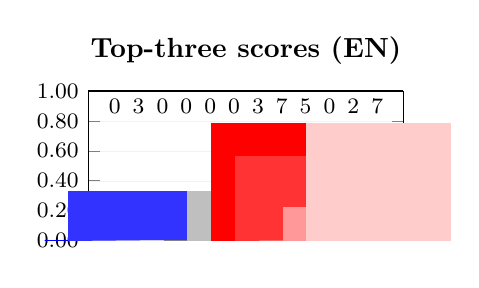
\begin{tikzpicture}[scale=1.0,every node/.style={scale=1.0}]
	\begin{axis}[
    		title=\textbf{Top-three scores (EN)},
		scale only axis,
		clip=false,
		separate axis lines,
		xtick={1,2,3,4,5,6,7,8,9,10,11,12},
        	x tick style={draw=none},
        	xticklabels={,,},
		width=4cm,height=1.9cm,
		tick label style={font=\footnotesize},
		xticklabel style={rotate=90},
		ymajorgrids,
    		grid style={line width=.1pt, draw=gray!10},
		ymin=0,ymax=1.0,
		every axis plot/.append style={
          		ybar,
          		bar width=6.0,
          		bar shift=0.5pt,
			fill
		},
		scaled y ticks=false,
		y tick label style={
        		/pgf/number format/.cd,
            		fixed,
            		fixed zerofill,
            		precision=2,
        		/tikz/.cd
    		}
	]

		\addplot[blue] coordinates {(1,0.00)};
     	 	\addplot[blue!80] coordinates {(2,0.33)};
      		\addplot[blue!60] coordinates {(3,0.00)};
      		\addplot[blue!40] coordinates {(4,0.00)};
		\addplot[blue!20] coordinates {(5,0.00)};
     	 	\addplot[gray] coordinates {(6,0.00)};
      		\addplot[lightgray] coordinates {(7,0.33)};
      		\addplot[red] coordinates {(8,0.78)};
     	 	\addplot[red!80] coordinates {(9,0.56)};
      		\addplot[red!60] coordinates {(10,0.00)};
      		\addplot[red!40] coordinates {(11,0.22)};
		\addplot[red!20] coordinates {(12,0.78)};

		\node at (axis cs: 1,0.9) {\footnotesize 0};
		\node at (axis cs: 2,0.9) {\footnotesize 3};
		\node at (axis cs: 3,0.9) {\footnotesize 0};
		\node at (axis cs: 4,0.9) {\footnotesize 0};
		\node at (axis cs: 5,0.9) {\footnotesize 0};
		\node at (axis cs: 6,0.9) {\footnotesize 0};
		\node at (axis cs: 7,0.9) {\footnotesize 3};
		\node at (axis cs: 8,0.9) {\footnotesize 7};
		\node at (axis cs: 9,0.9) {\footnotesize 5};
		\node at (axis cs: 10,0.9) {\footnotesize 0};
		\node at (axis cs: 11,0.9) {\footnotesize 2};
		\node at (axis cs: 12,0.9) {\footnotesize 7};
	\end{axis}
\end{tikzpicture}

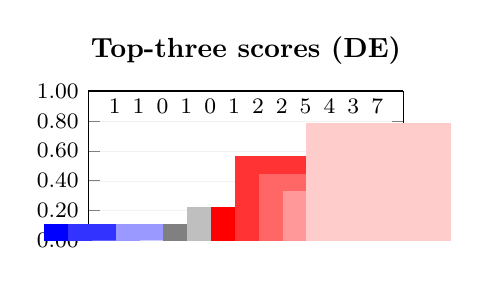
\begin{tikzpicture}[scale=1.0,every node/.style={scale=1.0}]
	\begin{axis}[
    		title=\textbf{Top-three scores (DE)},
		scale only axis,
		clip=false,
		separate axis lines,
		xtick={1,2,3,4,5,6,7,8,9,10,11,12},
        	x tick style={draw=none},
        	xticklabels={,,},
		width=4cm,height=1.9cm,
		tick label style={font=\footnotesize},
		xticklabel style={rotate=90},
		ymajorgrids,
    		grid style={line width=.1pt, draw=gray!10},
		ymin=0,ymax=1.0,
		every axis plot/.append style={
          		ybar,
          		bar width=6.0,
          		bar shift=0.5pt,
			fill
		},
		scaled y ticks=false,
		y tick label style={
        		/pgf/number format/.cd,
            		fixed,
            		fixed zerofill,
            		precision=2,
        		/tikz/.cd
    		}
	]

		\addplot[blue] coordinates {(1,0.11)};
     	 	\addplot[blue!80] coordinates {(2,0.11)};
      		\addplot[blue!60] coordinates {(3,0.00)};
      		\addplot[blue!40] coordinates {(4,0.11)};
		\addplot[blue!20] coordinates {(5,0.00)};
     	 	\addplot[gray] coordinates {(6,0.11)};
      		\addplot[lightgray] coordinates {(7,0.22)};
      		\addplot[red] coordinates {(8,0.22)};
     	 	\addplot[red!80] coordinates {(9,0.56)};
      		\addplot[red!60] coordinates {(10,0.44)};
      		\addplot[red!40] coordinates {(11,0.33)};
		\addplot[red!20] coordinates {(12,0.78)};

		\node at (axis cs: 1,0.9) {\footnotesize 1};
		\node at (axis cs: 2,0.9) {\footnotesize 1};
		\node at (axis cs: 3,0.9) {\footnotesize 0};
		\node at (axis cs: 4,0.9) {\footnotesize 1};
		\node at (axis cs: 5,0.9) {\footnotesize 0};
		\node at (axis cs: 6,0.9) {\footnotesize 1};
		\node at (axis cs: 7,0.9) {\footnotesize 2};
		\node at (axis cs: 8,0.9) {\footnotesize 2};
		\node at (axis cs: 9,0.9) {\footnotesize 5};
		\node at (axis cs: 10,0.9) {\footnotesize 4};
		\node at (axis cs: 11,0.9) {\footnotesize 3};
		\node at (axis cs: 12,0.9) {\footnotesize 7};
	\end{axis}
\end{tikzpicture}

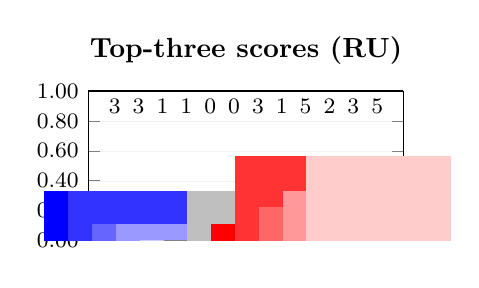
\begin{tikzpicture}[scale=1.0,every node/.style={scale=1.0}]
	\begin{axis}[
    		title=\textbf{Top-three scores (RU)},
		scale only axis,
		clip=false,
		separate axis lines,
		xtick={1,2,3,4,5,6,7,8,9,10,11,12},
        	x tick style={draw=none},
        	xticklabels={,,},
		width=4cm,height=1.9cm,
		tick label style={font=\footnotesize},
		xticklabel style={rotate=90},
		ymajorgrids,
    		grid style={line width=.1pt, draw=gray!10},
		ymin=0,ymax=1.0,
		every axis plot/.append style={
          		ybar,
          		bar width=6.0,
          		bar shift=0.5pt,
			fill
		},
		scaled y ticks=false,
		y tick label style={
        		/pgf/number format/.cd,
            		fixed,
            		fixed zerofill,
            		precision=2,
        		/tikz/.cd
    		}
	]

		\addplot[blue] coordinates {(1,0.33)};
     	 	\addplot[blue!80] coordinates {(2,0.33)};
      		\addplot[blue!60] coordinates {(3,0.11)};
      		\addplot[blue!40] coordinates {(4,0.11)};
		\addplot[blue!20] coordinates {(5,0.00)};
     	 	\addplot[gray] coordinates {(6,0.00)};
      		\addplot[lightgray] coordinates {(7,0.33)};
      		\addplot[red] coordinates {(8,0.11)};
     	 	\addplot[red!80] coordinates {(9,0.56)};
      		\addplot[red!60] coordinates {(10,0.22)};
      		\addplot[red!40] coordinates {(11,0.33)};
		\addplot[red!20] coordinates {(12,0.56)};

		\node at (axis cs: 1,0.9) {\footnotesize 3};
		\node at (axis cs: 2,0.9) {\footnotesize 3};
		\node at (axis cs: 3,0.9) {\footnotesize 1};
		\node at (axis cs: 4,0.9) {\footnotesize 1};
		\node at (axis cs: 5,0.9) {\footnotesize 0};
		\node at (axis cs: 6,0.9) {\footnotesize 0};
		\node at (axis cs: 7,0.9) {\footnotesize 3};
		\node at (axis cs: 8,0.9) {\footnotesize 1};
		\node at (axis cs: 9,0.9) {\footnotesize 5};
		\node at (axis cs: 10,0.9) {\footnotesize 2};
		\node at (axis cs: 11,0.9) {\footnotesize 3};
		\node at (axis cs: 12,0.9) {\footnotesize 5};
	\end{axis}
\end{tikzpicture}

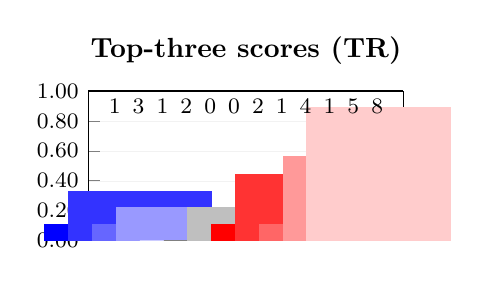
\begin{tikzpicture}[scale=1.0,every node/.style={scale=1.0}]
	\begin{axis}[
    		title=\textbf{Top-three scores (TR)},
		scale only axis,
		clip=false,
		separate axis lines,
		xtick={1,2,3,4,5,6,7,8,9,10,11,12},
        	x tick style={draw=none},
        	xticklabels={,,},
		width=4cm,height=1.9cm,
		tick label style={font=\footnotesize},
		xticklabel style={rotate=90},
		ymajorgrids,
    		grid style={line width=.1pt, draw=gray!10},
		ymin=0,ymax=1.0,
		every axis plot/.append style={
          		ybar,
          		bar width=6.0,
          		bar shift=0.5pt,
			fill
		},
		scaled y ticks=false,
		y tick label style={
        		/pgf/number format/.cd,
            		fixed,
            		fixed zerofill,
            		precision=2,
        		/tikz/.cd
    		}
	]

		\addplot[blue] coordinates {(1,0.11)};
     	 	\addplot[blue!80] coordinates {(2,0.33)};
      		\addplot[blue!60] coordinates {(3,0.11)};
      		\addplot[blue!40] coordinates {(4,0.22)};
		\addplot[blue!20] coordinates {(5,0.00)};
     	 	\addplot[gray] coordinates {(6,0.00)};
      		\addplot[lightgray] coordinates {(7,0.22)};
      		\addplot[red] coordinates {(8,0.11)};
     	 	\addplot[red!80] coordinates {(9,0.44)};
      		\addplot[red!60] coordinates {(10,0.11)};
      		\addplot[red!40] coordinates {(11,0.56)};
		\addplot[red!20] coordinates {(12,0.89)};
		
		\node at (axis cs: 1,0.9) {\footnotesize 1};
		\node at (axis cs: 2,0.9) {\footnotesize 3};
		\node at (axis cs: 3,0.9) {\footnotesize 1};
		\node at (axis cs: 4,0.9) {\footnotesize 2};
		\node at (axis cs: 5,0.9) {\footnotesize 0};
		\node at (axis cs: 6,0.9) {\footnotesize 0};
		\node at (axis cs: 7,0.9) {\footnotesize 2};
		\node at (axis cs: 8,0.9) {\footnotesize 1};
		\node at (axis cs: 9,0.9) {\footnotesize 4};
		\node at (axis cs: 10,0.9) {\footnotesize 1};
		\node at (axis cs: 11,0.9) {\footnotesize 5};
		\node at (axis cs: 12,0.9) {\footnotesize 8};
	\end{axis}
\end{tikzpicture}

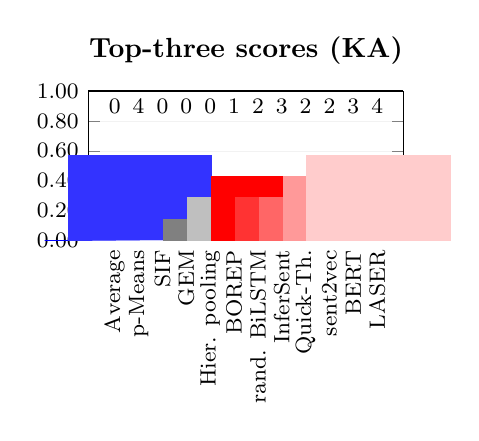
\begin{tikzpicture}[scale=1.0,every node/.style={scale=1.0}]
	\begin{axis}[
    		title=\textbf{Top-three scores (KA)},
		scale only axis,
		clip=false,
		separate axis lines,
		xtick={1,2,3,4,5,6,7,8,9,10,11,12},
        	x tick style={draw=none},
        	xticklabels={Average,p-Means,SIF,GEM,Hier. pooling,BOREP,rand. BiLSTM,InferSent,Quick-Th.,sent2vec,BERT,LASER},
		width=4cm,height=1.9cm,
		tick label style={font=\footnotesize},
		xticklabel style={rotate=90},
		ymajorgrids,
    		grid style={line width=.1pt, draw=gray!10},
		ymin=0,ymax=1.0,
		every axis plot/.append style={
          		ybar,
          		bar width=6.0,
          		bar shift=0.5pt,
			fill
		},
		scaled y ticks=false,
		y tick label style={
        		/pgf/number format/.cd,
            		fixed,
            		fixed zerofill,
            		precision=2,
        		/tikz/.cd
    		}
	]

		\addplot[blue] coordinates {(1,0.00)};
     	 	\addplot[blue!80] coordinates {(2,0.57)};
      		\addplot[blue!60] coordinates {(3,0.00)};
      		\addplot[blue!40] coordinates {(4,0.00)};
		\addplot[blue!20] coordinates {(5,0.00)};
     	 	\addplot[gray] coordinates {(6,0.14)};
      		\addplot[lightgray] coordinates {(7,0.29)};
      		\addplot[red] coordinates {(8,0.43)};
     	 	\addplot[red!80] coordinates {(9,0.29)};
      		\addplot[red!60] coordinates {(10,0.29)};
      		\addplot[red!40] coordinates {(11,0.43)};
		\addplot[red!20] coordinates {(12,0.57)};

		\node at (axis cs: 1,0.9) {\footnotesize 0};
		\node at (axis cs: 2,0.9) {\footnotesize 4};
		\node at (axis cs: 3,0.9) {\footnotesize 0};
		\node at (axis cs: 4,0.9) {\footnotesize 0};
		\node at (axis cs: 5,0.9) {\footnotesize 0};
		\node at (axis cs: 6,0.9) {\footnotesize 1};
		\node at (axis cs: 7,0.9) {\footnotesize 2};
		\node at (axis cs: 8,0.9) {\footnotesize 3};
		\node at (axis cs: 9,0.9) {\footnotesize 2};
		\node at (axis cs: 10,0.9) {\footnotesize 2};
		\node at (axis cs: 11,0.9) {\footnotesize 3};
		\node at (axis cs: 12,0.9) {\footnotesize 4};
	\end{axis}
\end{tikzpicture}


% Results measured by Accuracy
% -----------------------------------------------------------------------------------------------------------------------------------------------------
\subsection{Results measured by Accuracy}

\begin{table}[H]
	\centering
	\renewcommand{\arraystretch}{2.1}
	\begin{adjustbox}{angle=90}
	\scalebox{0.8}{
	\begin{tabularx}{1.125\textheight}{
		| l ? Y | c | Y | c ? Y | c | Y | c | Y | c | Y | c | Y | c ? Y | c | Y | c |
	}
	\hline
	\multicolumn{19}{| c |}{
		\cellcolor{tud9c}\textcolor{white}{
			\textbf{Language: English (Accuracy)}}} 			\\
	\hline

	\rowcolor{tud9c!85}
	\cellcolor{tud9c!85}										&
	\multicolumn{4}{ c ?}{\textbf{Surface Tasks}} 				& 
		\multicolumn{10}{ c ?}{\textbf{Syntactic Tasks}}		&
		\multicolumn{4}{c |}{\textbf{Semantic Tasks}}			\\

	\cellcolor{tud9c!85}										& 
		\multicolumn{2}{ c |}{
			\cellcolor{tud9c!70}\textbf{\caps{SentLen}}} 		&
		\multicolumn{2}{ c ?}{
			\cellcolor{tud9c!70}\textbf{\caps{WC}}} 			&
		\multicolumn{2}{ c |}{
			\cellcolor{tud9c!70}\textbf{\caps{BiShift}}}			&
		\multicolumn{2}{ c |}{
			\cellcolor{tud9c!70}\textbf{\caps{SVAgree}}} 		&
		\multicolumn{2}{ c |}{
			\cellcolor{tud9c!70}\textbf{\caps{SVDist}}} 			&
		\multicolumn{2}{ c |}{
			\cellcolor{tud9c!70}\textbf{\caps{Voice}}}			&
		\multicolumn{2}{ c ?}{
			\cellcolor{tud9c!70}\textbf{\caps{WO}}}			&
		\multicolumn{2}{ c |}{
			\cellcolor{tud9c!70}\textbf{\caps{EOS}}} 			&
		\multicolumn{2}{ c |}{
			\cellcolor{tud9c!70}\textbf{\caps{SubjNum}}}		\\

	\rowcolor{tud9c!55}
	\multirow{-3}{*}{\cellcolor{tud9c!85}\textbf{Embedding}}	&
		\textbf{F1} & \textbf{R} & \textbf{F1} & \textbf{R} & \textbf{F1} & \textbf{R} &
	   	\textbf{F1} & \textbf{R} & \textbf{F1} & \textbf{R} & \textbf{F1} & \textbf{R} &
	   	\textbf{F1} & \textbf{R} & \textbf{F1} & \textbf{R} & \textbf{F1} & \textbf{R} \\
	\hline\hline
	\multicolumn{19}{| l |}{\cellcolor{tud9c!30}\textbf{Size of the data set}} \\ \hline
	\# instances &
                10,000 	& - &
                10,000 	& - &
                10,000 	& - &
                10,000 	& - &
                10,000 	& - &
                9,999 		& - &
                10,000 	& - &
		   10,000 	& - &
                9,448 		& - \\    
	\hline\hline 
	\multicolumn{19}{| l |}{\cellcolor{tud9c!30}\textbf{Majority class (baseline)}} \\ \hline
	\rowcolor{lightgray!30}
	Majority &
                17.9 & - &
                13.3 & - &
                50.2 & - &
                51.1 & - &
                47.5 & - &
                61.0 & - &
                33.4 & - &
		   21.7 & - &
                75.7 & - \\
	\hline\hline   
	\multicolumn{19}{| l |}{\cellcolor{tud9c!30}\textbf{Random embeddings (baseline)}} \\ \hline
	\rowcolor{lightgray!30}
	BOREP &
                50.728 & 8 &
                65.800 & 10 &
                49.780 & 8 &
                79.680 & 7 &
                58.659 & 11 &
                79.490 & 7 &
                29.591 & 8 &
                27.780 & 6 &
                88.073 & 8 \\
        \hline
	  \rowcolor{lightgray!30}
        Random BiLSTM &
                62.730 & 4 &
                65.999 & 9 &
                51.880 & 6 &
                80.740 & 4 &
                66.110 & 4 &
                \cellcolor{bronze}{83.990} & \cellcolor{bronze}{3} &
                59.889 & 4 &
                \cellcolor{bronze}{31.101} & \cellcolor{bronze}{3} &
                \cellcolor{bronze}{91.174} & \cellcolor{bronze}{3} \\
	\hline\hline
	\multicolumn{19}{| l |}{\cellcolor{tud9c!30}\textbf{Average embeddings (\textit{FastText})}} \\ \hline
	Vanilla average &
                30.220 & 11 &
                75.919 & 8 &
                49.760 & 9 &
                77.430 & 9 &
                61.680 & 7 &
                80.820 & 6 &
                25.811 & 9 &
                24.510 & 10 &
                89.703 & 6 \\
        \hline
        p-Means &
                61.430 & 5 &
                76.119 & 7 &
                49.260 & 12 &
                79.820 & 6 &
                61.050 & 8 &
                82.140 & 4 &
                20.381 & 11 &
                28.880 & 5 &
                89.925 & 4 \\
        \hline
        SIF &
                28.061 & 12 &
                77.518 & 6 &
                49.430 & 11 &
                80.650 & 5 &
                60.810 & 9 &
                77.540 & 10 &
                24.890 & 10 &
                23.350 & 11 &
                88.380 & 7 \\
        \hline
        GEM &
                35.099 & 9 &
                82.572 & 4 &
                49.760 & 9 &
                78.510 & 8 &
                54.700 & 12 &
                73.550 & 12 &
                07.080 & 12 &
                25.770 & 7 &
                85.956 & 10 \\
        \hline
        hier. pooling &
                55.801 & 7 &
                55.287 & 12 &
                50.700 & 7 &
                65.890 & 11 &
                62.810 & 6 &
                78.980 & 9 &
                37.451 & 7 &
                30.080 & 4 &
                87.089 & 9 \\
	\hline\hline
	\multicolumn{19}{| l |}{\cellcolor{tud9c!30}\textbf{Trained embeddings}} \\ \hline
	InferSent &
                \cellcolor{bronze}{68.951} & \cellcolor{bronze}{3} &
                \cellcolor{gold}{94.780} & \cellcolor{gold}{1} &
                54.390 & 4 &
                \cellcolor{gold}{91.320} & \cellcolor{gold}{1} &
                \cellcolor{silver}{69.599} & \cellcolor{silver}{2} &
                \cellcolor{silver}{87.450} & \cellcolor{silver}{2} &
                \cellcolor{bronze}{76.050} & \cellcolor{bronze}{3} &
                25.050 & 8 &
                \cellcolor{silver}{91.311} & \cellcolor{silver}{2} \\
        \hline
        Quick-Thought &
                \cellcolor{silver}{68.970} & \cellcolor{silver}{2} &
                \cellcolor{bronze}{84.480} & \cellcolor{bronze}{3} &
                \cellcolor{bronze}{54.660} & \cellcolor{bronze}{3} &
                \cellcolor{bronze}{88.520} & \cellcolor{bronze}{3} &
                \cellcolor{bronze}{67.321} & \cellcolor{bronze}{3} &
                82.140 & 4 &
                \cellcolor{silver}{80.420} & \cellcolor{silver}{2} &
                24.959 & 9 &
                82.559 & 12 \\
        \hline
        sent2vec &
                31.000 & 10 &
                81.555 & 5 &
                53.190 & 5 &
                \cellcolor{silver}{90.900} & \cellcolor{silver}{2} &
                59.170 & 10 &
                79.090 & 8 &
                38.090 & 6 &
                22.640 & 12 &
                82.845 & 11 \\
        \hline
        BERT &
                59.169 & 6 &
                61.608 & 11 &
                \cellcolor{gold}{64.250} & \cellcolor{gold}{1} &
                72.260 & 10 &
                66.070 & 5 &
                77.360 & 11 &
                56.869 & 5 &
                \cellcolor{silver}{31.921} & \cellcolor{silver}{2} &
                89.713 & 5 \\
        \hline
        LASER &
                \cellcolor{gold}{74.971} & \cellcolor{gold}{1} &
                \cellcolor{silver}{89.979} & \cellcolor{silver}{2} &
                \cellcolor{silver}{59.950} & \cellcolor{silver}{2} &
                57.120 & 12 &
                \cellcolor{gold}{72.921} & \cellcolor{gold}{1} &
                \cellcolor{gold}{90.920} & \cellcolor{gold}{1} &
                \cellcolor{gold}{84.790} & \cellcolor{gold}{1} &
                \cellcolor{gold}{37.790} & \cellcolor{gold}{1} &
                \cellcolor{gold}{92.909} & \cellcolor{gold}{1} \\
	\hline
	\end{tabularx}}
	\end{adjustbox}
	\caption[Probing task results for the English language (accuracy)]{Probing task results for the English language (accuracy).}
	\label{tab:results_probing_tasks_en_acc}
\end{table}	


% Detailed Downstream Task Results
% -----------------------------------------------------------------------------------------------------------------------------------------------------
\section{Detailed Downstream Task Results}
\label{sec:appendix_downstream}

% Results measured by F1 Score
% -----------------------------------------------------------------------------------------------------------------------------------------------------
\subsection{Results measured by F1 Score}

\begin{table}[H]
	\centering
	\renewcommand{\arraystretch}{1.5}
	\begin{adjustbox}{angle=90}
	\scalebox{0.72}{
	\begin{tabular}{
		| l ? >{\centering}m{2.4cm} | c ? >{\centering}m{2.4cm} | c ? >{\centering}m{2.4cm} | c |
	}
	\hline
	\multicolumn{7}{| c |}{
		\cellcolor{tud9c}\textcolor{white}{
			\textbf{Language: English (F1)}}}					\\
	\hline

	\cellcolor{tud9c!85}										& 
		\multicolumn{2}{ c ?}{
			\cellcolor{tud9c!70}\textbf{\caps{ArgMin}}}			&
		\multicolumn{2}{ c ?}{
			\cellcolor{tud9c!70}\textbf{\caps{Senti}}}			&
		\multicolumn{2}{ c |}{
			\cellcolor{tud9c!70}\textbf{\caps{TREC}}}			\\

	\rowcolor{tud9c!55}
	\multirow{-3}{*}{\cellcolor{tud9c!85}\textbf{Embedding}}	&
		\textbf{F1} & \textbf{R} & \textbf{F1} & \textbf{R} & \textbf{F1} & \textbf{R} \\
	\hline\hline
	\multicolumn{7}{| l |}{\cellcolor{tud9c!30}\textbf{Size of the data set}} \\ \hline
	\# instances &
                25,303 	& - &
                14,148 	& - &
                5,952 		& - \\
	\hline\hline 
	\multicolumn{7}{| l |}{\cellcolor{tud9c!30}\textbf{Majority class (baseline)}} \\ \hline
	\rowcolor{lightgray!30}
	Majority &
                56.4 & - &
                64.0 & - &
                22.6 & - \\
	\hline\hline   
	\multicolumn{7}{| l |}{\cellcolor{tud9c!30}\textbf{Random embeddings (baseline)}} \\ \hline
	\rowcolor{lightgray!30}
	BOREP &
                00.542 & 13 &
                00.646 & 9 &
                00.819 & 5 \\
        \hline
	 \rowcolor{lightgray!30}
        Random BiLSTM &
                00.536 & 15 &
                00.688 & 6 &
                00.774 & 9 \\
	\hline\hline
	\multicolumn{7}{| l |}{\cellcolor{tud9c!30}\textbf{Average embeddings (\textit{FastText})}} \\ \hline
	Vanilla average &
                00.550 & 12 &
                00.698 & 4 &
                00.795 & 7 \\
        \hline
        p-Means &
                00.568 & 7 &
                00.695 & 5 &
                00.767 & 10 \\
        \hline
        SIF &
                00.533 & 16 &
                \cellcolor{silver}{00.702} & \cellcolor{silver}{2} &
                00.715 & 13 \\
        \hline
        GEM &
                00.540 & 14 &
                00.646 & 9 &
                00.820 & 4 \\
        \hline
        hier. pooling &
                00.513 & 17 &
                00.627 & 16 &
                00.724 & 12 \\
	\hline\hline
	\multicolumn{7}{| l |}{\cellcolor{tud9c!30}\textbf{Average embeddings (\textit{word2vec})}} \\ \hline
	Vanilla average &
                00.585 & 4 &
                00.639 & 12 &
                00.693 & 16 \\
        \hline
        p-Means &
                00.561 & 9 &
                00.622 & 18 &
                00.713 & 14 \\
        \hline
        SIF &
                00.581 & 5 &
                00.627 & 16 &
                00.644 & 18 \\
        \hline
        GEM &
                00.426 & 22 &
                00.516 & 22 &
                00.576 & 20 \\
        \hline
        hier. pooling &
                00.555 & 11 &
                00.603 & 19 &
                00.697 & 15 \\
	\hline\hline
	\multicolumn{7}{| l |}{\cellcolor{tud9c!30}\textbf{Average embeddings (\textit{Attract-Repel})}} \\ \hline
	Vanilla average &
                00.511 & 18&
                00.630 & 15 &
                00.651 & 17 \\
        \hline
        p-Means &
                00.568 & 7 &
                00.660 & 7 &
                00.748 & 11 \\
        \hline
        SIF &
                00.497 & 19 &
                00.631 & 14 &
                00.554 & 22 \\
        \hline
        GEM &
                00.487 & 21 &
                00.565 & 21 &
                00.564 & 21 \\
        \hline
        hier. pooling &
                00.492 & 20 &
                00.594 & 20 &
                00.641 & 19 \\
	\hline\hline
	\multicolumn{7}{| l |}{\cellcolor{tud9c!30}\textbf{Trained embeddings}} \\ \hline
	InferSent &
                \cellcolor{silver}{00.604} & \cellcolor{silver}{2} &
                \cellcolor{silver}{00.702} & \cellcolor{silver}{2} &
                \cellcolor{gold}{00.920} & \cellcolor{gold}{1} \\
        \hline
        Quick-Thought &
                00.581 & 5 &
                00.636 & 13 &
                00.814 & 6 \\
        \hline
        sent2vec &
                \cellcolor{gold}{00.608} & \cellcolor{gold}{1} &
                00.656 & 8 &
                00.792 & 8 \\
        \hline
        BERT &
                00.558 & 10 &
                00.644 & 11 &
                \cellcolor{silver}{00.876} & \cellcolor{silver}{2} \\
        \hline
        LASER &
                \cellcolor{bronze}{00.596} & \cellcolor{bronze}{3} &
                \cellcolor{gold}{00.727} & \cellcolor{gold}{1} &
                \cellcolor{bronze}{00.851} & \cellcolor{bronze}{3} \\
	\hline
	\end{tabular}}
	\end{adjustbox}
	\caption[Downstream task results for the English language (F1 scores)]{Downstream task results for the English language (F1 scores).}
	\label{tab:downstream_probing_tasks_en}
\end{table}	
\begin{table}[H]
	\centering
	\renewcommand{\arraystretch}{1.5}
	\begin{adjustbox}{angle=90}
	\scalebox{0.72}{
	\begin{tabular}{
		| l ? >{\centering}m{2.4cm} | c ? >{\centering}m{2.4cm} | c ? >{\centering}m{2.4cm} | c |
	}
	\hline
	\multicolumn{7}{| c |}{
		\cellcolor{tud9c}\textcolor{white}{
			\textbf{Language: German (F1)}}} 					\\
	\hline

	\cellcolor{tud9c!85}										& 
		\multicolumn{2}{ c ?}{
			\cellcolor{tud9c!70}\textbf{\caps{ArgMin}}} 		&
		\multicolumn{2}{ c ?}{
			\cellcolor{tud9c!70}\textbf{\caps{Senti}}}			&
		\multicolumn{2}{ c |}{
			\cellcolor{tud9c!70}\textbf{\caps{TREC}}}			\\

	\rowcolor{tud9c!55}
	\multirow{-3}{*}{\cellcolor{tud9c!85}\textbf{Embedding}}	&
		\textbf{F1} & \textbf{R} & \textbf{F1} & \textbf{R} & \textbf{F1} & \textbf{R} \\
	\hline\hline
	\multicolumn{7}{| l |}{\cellcolor{tud9c!30}\textbf{Size of the data set}} \\ \hline
	\# instances &
                25,303 	& - &
                17,908 	& - &
                5,952 	& - \\
	\hline\hline 
	\multicolumn{7}{| l |}{\cellcolor{tud9c!30}\textbf{Majority class (baseline)}} \\ \hline
	\rowcolor{lightgray!30}
	Majority &
                56.4 & - &
                67.8 & - &
                22.6 & - \\
	\hline\hline   
	\multicolumn{7}{| l |}{\cellcolor{tud9c!30}\textbf{Random embeddings (baseline)}} \\ \hline
	\rowcolor{lightgray!30}
	BOREP &
                00.507 & 7 &
                00.545 & 8 &
                00.764 & 4 \\
        \hline
	\rowcolor{lightgray!30}
        Random BiLSTM &
                00.507 & 7 &
                00.559 & 4 &
                00.676 & 9 \\
	\hline\hline
	\multicolumn{7}{| l |}{\cellcolor{tud9c!30}\textbf{Average embeddings (\textit{FastText})}} \\ \hline
	Vanilla average &
                00.507 & 7 &
                00.544 & 9 &
                00.694 & 8 \\
        \hline
        p-Means &
                \cellcolor{silver}{00.534} & \cellcolor{silver}{2} &
                00.550 & 6 &
                \cellcolor{bronze}{00.765} & \cellcolor{bronze}{3} \\
        \hline
        SIF &
                00.514 & 6 &
                00.555 & 5 &
                00.734 & 6 \\
        \hline
        GEM &
                00.521 & 4 &
                \cellcolor{bronze}{00.572} & \cellcolor{bronze}{3} &
                00.730 & 7 \\
        \hline
        hier. pooling &
                00.467 & 16 &
                00.489 & 18 &
                00.601 & 12 \\
	\hline\hline
	\multicolumn{7}{| l |}{\cellcolor{tud9c!30}\textbf{Average embeddings (\textit{word2vec})}} \\ \hline
	Vanilla average &
                00.501 & 11 &
                00.532 & 11 &
                00.581 & 14 \\
        \hline
        p-Means &
                00.479 & 14 &
                00.540 & 10 &
                00.596 & 13 \\
        \hline
        SIF &
                00.499 & 12 &
                00.515 & 14 &
                00.558 & 17 \\
        \hline
        GEM &
                00.391 & 22 &
                00.478 & 19 &
                00.553 & 18 \\
        \hline
        hier. pooling &
                00.471 & 15 &
                00.520 & 13 &
                00.569 & 16 \\
	\hline\hline
	\multicolumn{7}{| l |}{\cellcolor{tud9c!30}\textbf{Average embeddings (\textit{Attract-Repel})}} \\ \hline
	Vanilla average &
                00.432 & 20 &
                00.466 & 20 &
                00.488 & 21 \\
        \hline
        p-Means &
                00.505 & 10 &
                00.529 & 12 &
                00.607 & 11 \\
        \hline
        SIF &
                00.423 & 21 &
                00.461 & 21 &
                00.489 & 20 \\
        \hline
        GEM &
                00.443 & 18 &
                00.506 & 17 &
                00.491 & 19 \\
        \hline
        hier. pooling &
                00.434 & 19 &
                00.432 & 22 &
                00.408 & 22 \\

	\hline\hline
	\multicolumn{7}{| l |}{\cellcolor{tud9c!30}\textbf{Trained embeddings}} \\ \hline
	InferSent &
                00.456 & 17 &
                00.547 & 7 &
                00.580 & 15 \\
        \hline
        Quick-Thought &
                00.497 & 13 &
                00.511 & 16 &
                00.667 & 10 \\
        \hline
        sent2vec &
                \cellcolor{silver}{00.534} & \cellcolor{silver}{2} &
                \cellcolor{silver}{00.590} & \cellcolor{silver}{2} &
                \cellcolor{gold}{00.846} & \cellcolor{gold}{1} \\
        \hline
        BERT &
                00.517 & 5 &
                00.514 & 15 &
                \cellcolor{silver}{00.802} & \cellcolor{silver}{2} \\
        \hline
        LASER &
                \cellcolor{gold}{00.583} & \cellcolor{gold}{1} &
                \cellcolor{gold}{00.623} & \cellcolor{gold}{1} &
                00.753 & 5 \\
	\hline
	\end{tabular}}
	\end{adjustbox}
	\caption[Downstream task results for the German language (F1 scores)]{Downstream task results for the German language (F1 scores).}
	\label{tab:downstream_probing_tasks_de}
\end{table}
\begin{table}[H]
	\centering
	\renewcommand{\arraystretch}{1.5}
	\begin{adjustbox}{angle=90}
	\scalebox{0.72}{
	\begin{tabular}{
		| l ? >{\centering}m{2.7cm} | c ? >{\centering}m{2.7cm} | c ? >{\centering}m{2.7cm} | c |
	}
	\hline
	\multicolumn{7}{| c |}{
		\cellcolor{tud9c}\textcolor{white}{
			\textbf{Language: Russian (F1)}}} 					\\
	\hline

	\cellcolor{tud9c!85}										& 
		\multicolumn{2}{ c ?}{
			\cellcolor{tud9c!70}\textbf{\caps{ArgMin}}} 		&
		\multicolumn{2}{ c ?}{
			\cellcolor{tud9c!70}\textbf{\caps{Senti}}}			&
		\multicolumn{2}{ c |}{
			\cellcolor{tud9c!70}\textbf{\caps{TREC}}}			\\

	\rowcolor{tud9c!55}
	\multirow{-3}{*}{\cellcolor{tud9c!85}\textbf{Embedding}}	&
		\textbf{F1} & \textbf{R} & \textbf{F1} & \textbf{R} & \textbf{F1} & \textbf{R} \\
	\hline\hline
	\multicolumn{7}{| l |}{\cellcolor{tud9c!30}\textbf{Size of the data set}} \\ \hline
	\# instances &
                25,303 	& - &
                30,000 	& - &
                5,952 		& - \\  
	\hline\hline 
	\multicolumn{7}{| l |}{\cellcolor{tud9c!30}\textbf{Majority class (baseline)}} \\ \hline
	\rowcolor{lightgray!30}
	Majority &
                56.4 & - &
                51.2 & - &
                22.6 & - \\
	\hline\hline   
	\multicolumn{7}{| l |}{\cellcolor{tud9c!30}\textbf{Random embeddings (baseline)}} \\ \hline
	\rowcolor{lightgray!30}
	 BOREP &
                00.518 & 11 &
                00.643 & 9 &
                00.778 & 7 \\
        \hline
        \rowcolor{lightgray!30}
        Random BiLSTM &
                00.521 & 10 &
                00.695 & 4 &
                00.739 & 10 \\
	\hline\hline
	\multicolumn{7}{| l |}{\cellcolor{tud9c!30}\textbf{Average embeddings (\textit{FastText})}} \\ \hline
	Vanilla average &
                00.535 & 4 &
                \cellcolor{silver}{00.703} & \cellcolor{silver}{2} &
                00.767 & 8 \\
        \hline
        p-Means &
                \cellcolor{silver}{00.553} & \cellcolor{silver}{2} &
                00.695 & 4 &
                00.799 & 5 \\
        \hline
        SIF &
                00.508 & 13 &
                \cellcolor{bronze}{00.701} & \cellcolor{bronze}{3} &
                00.731 & 13 \\
        \hline
        GEM &
                00.515 & 12 &
                00.630 & 10 &
                \cellcolor{bronze}{00.803} & \cellcolor{bronze}{3} \\
        \hline
        hier. pooling &
                00.486 & 16 &
                00.673 & 7 &
                00.717 & 15 \\
	\hline\hline
	\multicolumn{7}{| l |}{\cellcolor{tud9c!30}\textbf{Average embeddings (\textit{word2vec})}} \\ \hline
	Vanilla average &
                00.531 & 6 &
                00.601 & 14 &
                00.738 & 11 \\
        \hline
        p-Means &
                00.524 & 9 &
                00.605 & 13 &
                00.801 & 4 \\
        \hline
        SIF &
                00.529 & 8 &
                00.598 & 15 &
                00.732 & 12 \\
        \hline
        GEM &
                00.386 & 20 &
                00.551 & 22 &
                00.546 & 18 \\
        \hline
        hier. pooling &
                00.501 & 14 &
                00.584 & 17 &
                00.745 & 9 \\
	\hline\hline
	\multicolumn{7}{| l |}{\cellcolor{tud9c!30}\textbf{Average embeddings (\textit{Attract-Repel})}} \\ \hline
	Vanilla average &
                00.371 & 21 &
                00.568 & 21 &
                00.399 & 21 \\
        \hline
        p-Means &
                00.478 & 17 &
                00.586 & 16 &
                00.551 & 17 \\
        \hline
        SIF &
                00.365 & 22 &
                00.582 & 18 &
                00.394 & 22 \\
        \hline
        GEM &
                00.433 & 18 &
                00.578 & 19 &
                00.405 & 20 \\
        \hline
        hier. pooling &
                00.409 & 19 &
                00.574 & 20 &
                00.410 & 19 \\
	\hline\hline
	\multicolumn{7}{| l |}{\cellcolor{tud9c!30}\textbf{Trained embeddings}} \\ \hline
	InferSent &
                00.487 & 15 &
                00.676 & 6 &
                00.623 & 16 \\
        \hline
        Quick-Thought &
               \cellcolor{bronze}{00.540} & \cellcolor{bronze}{3} &
                00.627 & 11 &
                00.780 & 6 \\
        \hline
        sent2vec &
                00.534 & 5 &
                00.622 & 12 &
                \cellcolor{gold}{00.832} & \cellcolor{gold}{1} \\
        \hline
        BERT &
                00.531 & 6 &
                00.644 & 8 &
                \cellcolor{silver}{00.822} & \cellcolor{silver}{2} \\
        \hline
        LASER &
                \cellcolor{gold}{00.582} & \cellcolor{gold}{1} &
                \cellcolor{gold}{00.728} & \cellcolor{gold}{1} &
                00.728 & 14 \\
	\hline
	\end{tabular}}
	\end{adjustbox}
	\caption[Downstream task results for the Russian language (F1 scores)]{Downstream task results for the Russian language (F1 scores).}
	\label{tab:downstream_probing_tasks_ru}
\end{table}	
\begin{table}[H]
	\centering
	\renewcommand{\arraystretch}{1.5}
	\begin{adjustbox}{angle=90}
	\scalebox{0.72}{
	\begin{tabular}{
		| l ? >{\centering}m{2.7cm} | c ? >{\centering}m{2.7cm} | c ? >{\centering}m{2.7cm} | c |
	}
	\hline
	\multicolumn{7}{| c |}{
		\cellcolor{tud9c}\textcolor{white}{
			\textbf{Language: Turkish (F1)}}} 					\\
	\hline

	\cellcolor{tud9c!85}										& 
		\multicolumn{2}{ c ?}{
			\cellcolor{tud9c!70}\textbf{\caps{ArgMin}}} 		&
		\multicolumn{2}{ c ?}{
			\cellcolor{tud9c!70}\textbf{\caps{Senti}}}			&
		\multicolumn{2}{ c |}{
			\cellcolor{tud9c!70}\textbf{\caps{TREC}}}			\\

	\rowcolor{tud9c!55}
	\multirow{-3}{*}{\cellcolor{tud9c!85}\textbf{Embedding}}	&
		\textbf{F1} & \textbf{R} & \textbf{F1} & \textbf{R} & \textbf{F1} & \textbf{R} \\
	\hline\hline
	\multicolumn{7}{| l |}{\cellcolor{tud9c!30}\textbf{Size of the data set}} \\ \hline
	\# instances &
                25,303 	& - &
                6,172 		& - &
                5,952 		& - \\  
	\hline\hline 
	\multicolumn{7}{| l |}{\cellcolor{tud9c!30}\textbf{Majority class (baseline)}} \\ \hline
	\rowcolor{lightgray!30}
	Majority &
                56.4 & - &
                52.0 & - &
                22.6 & - \\
	\hline\hline   
	\multicolumn{7}{| l |}{\cellcolor{tud9c!30}\textbf{Random embeddings (baseline)}} \\ \hline
	\rowcolor{lightgray!30}
	 BOREP &
                00.512 & 10 &
                00.498 & 8 &
                \cellcolor{gold}{00.722} & \cellcolor{gold}{1} \\
        \hline
        \rowcolor{lightgray!30}
        Random BiLSTM &
                00.515 & 7 &
                \cellcolor{gold}{00.529} & \cellcolor{gold}{1} &
                00.685 & 6 \\
	\hline\hline
	\multicolumn{7}{| l |}{\cellcolor{tud9c!30}\textbf{Average embeddings (\textit{FastText})}} \\ \hline
	Vanilla average &
                00.525 & 4 &
                \cellcolor{gold}{00.529} & \cellcolor{gold}{1} &
                00.649 & 13 \\
        \hline
        p-Means &
                \cellcolor{silver}{00.547} & \cellcolor{silver}{2} &
                00.511 & 7 &
                00.683 & 7 \\
        \hline
        SIF &
                00.506 & 14 &
                \cellcolor{bronze}{00.528} & \cellcolor{bronze}{3} &
                00.658 & 11 \\
        \hline
        GEM &
                00.508 & 13 &
                00.513 & 6 &
                \cellcolor{silver}{00.715} & \cellcolor{silver}{2} \\
        \hline
        hier. pooling &
                00.509 & 12 &
                00.497 & 9 &
                00.626 & 15 \\
	\hline\hline
	\multicolumn{7}{| l |}{\cellcolor{tud9c!30}\textbf{Average embeddings (\textit{word2vec})}} \\ \hline
	Vanilla average &
                00.517 & 6 &
                00.479 & 13 &
                \cellcolor{bronze}{00.710} & \cellcolor{bronze}{3} \\
        \hline
        p-Means &
                00.513 & 9 &
                00.464 & 19 &
                00.683 & 7 \\
        \hline
        SIF &
                00.520 & 5 &
                00.477 & 15 &
                00.642 & 14 \\
        \hline
        GEM &
                00.386 & 22 &
                00.415 & 21 &
                00.546 & 20 \\
        \hline
        hier. pooling &
                00.503 & 16 &
                00.479 & 13 &
                00.623 & 16 \\
	\hline\hline
	\multicolumn{7}{| l |}{\cellcolor{tud9c!30}\textbf{Average embeddings (\textit{Attract-Repel})}} \\ \hline
	Vanilla average &
                00.476 & 19 &
                00.465 & 18 &
                00.599 & 17 \\
        \hline
        p-Means &
                \cellcolor{bronze}{00.540} & \cellcolor{bronze}{3} &
                00.487 & 10 &
                00.660 & 9 \\
        \hline
        SIF &
                00.466 & 20 &
                00.457 & 20 &
                00.597 & 18 \\
        \hline
        GEM &
                00.435 & 21 &
                00.411 & 22 &
                00.397 & 22 \\
        \hline
        hier. pooling &
                00.477 & 18 &
                00.472 & 16 &
                00.586 & 19 \\
	\hline\hline
	\multicolumn{7}{| l |}{\cellcolor{tud9c!30}\textbf{Trained embeddings}} \\ \hline
	InferSent &
                00.510 & 11 &
                00.514 & 5 &
                00.545 & 21 \\
        \hline
        Quick-Thought &
                00.515 & 7 &
                00.469 & 17 &
                00.650 & 12 \\
        \hline
        sent2vec &
                00.504 & 15 &
                00.483 & 12 &
                00.698 & 4 \\
        \hline
        BERT &
                00.493 & 17 &
                00.484 & 11 &
                00.695 & 5 \\
        \hline
        LASER &
                \cellcolor{gold}{00.555} & \cellcolor{gold}{1} &
                00.523 & 4 &
                00.660 & 9 \\
	\hline
	\end{tabular}}
	\end{adjustbox}
	\caption[Downstream task results for the Turkish language (F1 scores)]{Downstream task results for the Turkish language (F1 scores).}
	\label{tab:downstream_probing_tasks_tr}
\end{table}	
\begin{table}[H]
	\centering
	\renewcommand{\arraystretch}{1.5}
	\begin{adjustbox}{angle=90}
	\scalebox{0.72}{
	\begin{tabular}{
		| l ? >{\centering}m{2.4cm} | c ? >{\centering}m{2.4cm} | c ? >{\centering}m{2.4cm} | c |
	}
	\hline
	\multicolumn{7}{| c |}{
		\cellcolor{tud9c}\textcolor{white}{
			\textbf{Language: Georgian (F1)}}} 				\\
	\hline

	\cellcolor{tud9c!85}										& 
		\multicolumn{2}{ c ?}{
			\cellcolor{tud9c!70}\textbf{\caps{ArgMin}}} 		&
		\multicolumn{2}{ c ?}{
			\cellcolor{tud9c!70}\textbf{\caps{Senti}}}			&
		\multicolumn{2}{ c |}{
			\cellcolor{tud9c!70}\textbf{\caps{TREC}}}			\\

	\rowcolor{tud9c!55}
	\multirow{-3}{*}{\cellcolor{tud9c!85}\textbf{Embedding}}	&
		\textbf{F1} & \textbf{R} & \textbf{F1} & \textbf{R} & \textbf{F1} & \textbf{R} \\
	\hline\hline
	\multicolumn{7}{| l |}{\cellcolor{tud9c!30}\textbf{Size of the data set}} \\ \hline
	\# instances &
                25,303 	& - &
                11,513 	& - &
                5,952 		& - \\ 
	\hline\hline 
	\multicolumn{7}{| l |}{\cellcolor{tud9c!30}\textbf{Majority class (baseline)}} \\ \hline
	\rowcolor{lightgray!30}
	Majority &
                56.4 & - &
                54.8 & - &
                22.6 & - \\
	\hline\hline   
	\multicolumn{7}{| l |}{\cellcolor{tud9c!30}\textbf{Random embeddings (baseline)}} \\ \hline
	\rowcolor{lightgray!30}
	BOREP &
                \cellcolor{silver}{00.517} & \cellcolor{silver}{2} &
                00.544 & 4 &
                00.774 & 6 \\
        \hline
	 \rowcolor{lightgray!30}
        Random BiLSTM &
                00.506 & 4 &
                \cellcolor{bronze}{00.546} & \cellcolor{bronze}{3} &
                00.770 & 8 \\
	\hline\hline
	\multicolumn{7}{| l |}{\cellcolor{tud9c!30}\textbf{Average embeddings (\textit{FastText})}} \\ \hline
	Vanilla average &
                00.500 & 6 &
                00.514 & 7 &
                00.739 & 11 \\
        \hline
        p-Means &
                \cellcolor{gold}{00.541} & \cellcolor{gold}{1} &
                00.539 & 5 &
                00.774 & 6 \\
        \hline
        SIF &
                00.481 & 9 &
                00.511 & 8 &
                00.732 & 12 \\
        \hline
        GEM &
                00.500 & 6 &
                \cellcolor{gold}{00.596} & \cellcolor{gold}{1} &
                00.742 & 10 \\
        \hline
        hier. pooling &
                00.460 & 16 &
                00.474 & 14 &
                00.747 & 9 \\
	\hline\hline
	\multicolumn{7}{| l |}{\cellcolor{tud9c!30}\textbf{Average embeddings (\textit{word2vec})}} \\ \hline
	Vanilla average &
                00.480 & 10 &
                00.423 & 19 &
                00.684 & 16 \\
        \hline
        p-Means &
                00.480 & 10 &
                \cellcolor{silver}{00.568} & \cellcolor{silver}{2} &
                \cellcolor{bronze}{00.796} & \cellcolor{bronze}{3} \\
        \hline
        SIF &
                00.473 & 14 &
                00.406 & 21 &
                00.671 & 19 \\
        \hline
        GEM &
                00.388 & 22 &
                00.477 & 13 &
                00.673 & 18 \\
        \hline
        hier. pooling &
                00.475 & 13 &
                00.465 & 15 &
                00.723 & 14 \\
	\hline\hline
	\multicolumn{7}{| l |}{\cellcolor{tud9c!30}\textbf{Average embeddings (\textit{Attract-Repel})}} \\ \hline
	Vanilla average &
                00.460 & 16 &
                00.401 & 22 &
                00.705 & 15 \\
        \hline
        p-Means &
                \cellcolor{bronze}{00.512} & \cellcolor{bronze}{3} &
                00.484 & 12 &
                \cellcolor{gold}{00.841} & \cellcolor{gold}{1} \\
        \hline
        SIF &
                00.429 & 21 &
                00.418 & 20 &
                00.730 & 13 \\
        \hline
        GEM &
                00.434 & 20 &
                00.443 & 17 &
                00.619 & 20 \\
        \hline
        hier. pooling &
                00.450 & 18 &
                00.432 & 18 &
                00.684 & 16 \\
	\hline\hline
	\multicolumn{7}{| l |}{\cellcolor{tud9c!30}\textbf{Trained embeddings}} \\ \hline
	InferSent &
                00.479 & 12 &
                00.510 & 10 &
                00.578 & 21 \\
        \hline
        Quick-Thought &
                00.482 & 8 &
                00.488 & 11 &
                \cellcolor{silver}{00.811} & \cellcolor{silver}{2} \\
        \hline
        sent2vec &
                00.472 & 15 &
                00.531 & 6 &
                00.787 & 4 \\
        \hline
        BERT &
                00.502 & 5 &
                00.511 & 8 &
                00.784 & 5 \\
        \hline
        LASER &
                00.449 & 19 &
                00.450 & 16 &
                00.523 & 22 \\
	\hline
	\end{tabular}}
	\end{adjustbox}
	\caption[Downstream task results for the Georgian language (F1 scores)]{Downstream task results for the Georgian language (F1 scores).}
	\label{tab:downstream_probing_tasks_ka}
\end{table}	

\newpage

% Results measured by Accuracy
% -----------------------------------------------------------------------------------------------------------------------------------------------------
\subsection{Results measured by Accuracy}

\begin{table}[H]
	\centering
	\renewcommand{\arraystretch}{2.4}
	\begin{adjustbox}{angle=90}
	\scalebox{0.7}{
	\begin{tabular}{
		| l ? >{\centering}m{2.7cm} | c ? >{\centering}m{2.7cm} | c ? >{\centering}m{2.7cm} | c |
	}
	\hline
	\multicolumn{7}{| c |}{
		\cellcolor{tud9c}\textcolor{white}{
			\textbf{Language: English (Accuracy)}}}			\\
	\hline

	\cellcolor{tud9c!85}										& 
		\multicolumn{2}{ c ?}{
			\cellcolor{tud9c!70}\textbf{\caps{ArgMin}}}			&
		\multicolumn{2}{ c ?}{
			\cellcolor{tud9c!70}\textbf{\caps{Senti}}}			&
		\multicolumn{2}{ c |}{
			\cellcolor{tud9c!70}\textbf{\caps{TREC}}}			\\

	\rowcolor{tud9c!55}
	\multirow{-3}{*}{\cellcolor{tud9c!85}\textbf{Embedding}}	&
		\textbf{F1} & \textbf{R} & \textbf{F1} & \textbf{R} & \textbf{F1} & \textbf{R} \\
	\hline\hline
	\multicolumn{7}{| l |}{\cellcolor{tud9c!30}\textbf{Size of the data set}} \\ \hline
	\# instances &
                25,303 	& - &
                14,148 	& - &
                5,952 		& - \\
	\hline\hline 
	\multicolumn{7}{| l |}{\cellcolor{tud9c!30}\textbf{Majority class (baseline)}} \\ \hline
	\rowcolor{lightgray!30}
	Majority &
                56.4 & - &
                64.0 & - &
                22.6 & - \\
	\hline\hline   
	\multicolumn{7}{| l |}{\cellcolor{tud9c!30}\textbf{Random embeddings (baseline)}} \\ \hline
	\rowcolor{lightgray!30}
	BOREP &
                63.030 & 10 &
                74.366 & 7 &
                84.500 & 4 \\
        \hline
        \rowcolor{lightgray!30}
        Random BiLSTM &
                63.282 & 9 &
                77.200 & 5 &
                79.600 & 7 \\
	\hline\hline
	\multicolumn{7}{| l |}{\cellcolor{tud9c!30}\textbf{Average embeddings (\textit{FastText})}} \\ \hline
	Vanilla average &
                65.191 & 5 &
                \cellcolor{bronze}{78.380} & \cellcolor{bronze}{3} &
                79.600 & 7 \\
        \hline
        p-Means &
                64.709 & 6 &
                77.695 & 4 &
                81.800 & 5 \\
        \hline
        SIF &
                63.516 & 8 &
                \cellcolor{silver}{78.521} & \cellcolor{silver}{2} &
                76.200 & 11 \\
        \hline
        GEM &
                61.484 & 12 &
                72.267 & 12 &
                78.800 & 9 \\
        \hline
        hier. pooling &
                62.385 & 11 &
                74.288 & 8 &
                76.000 & 12 \\
	\hline\hline
	\multicolumn{7}{| l |}{\cellcolor{tud9c!30}\textbf{Trained embeddings}} \\ \hline
	InferSent &
                \cellcolor{bronze}{67.321} & \cellcolor{bronze}{3} &
                77.157 & 6 &
                \cellcolor{gold}{91.400} & \cellcolor{gold}{1} \\
        \hline
        Quick-Thought &
                66.235 & 4 &
                73.016 & 10 &
                81.400 & 6 \\
        \hline
        sent2vec &
                \cellcolor{silver}{67.693} & \cellcolor{silver}{2} &
                74.125 & 9 &
                78.200 & 10 \\
        \hline
        BERT &
                63.642 & 7 &
                73.002 & 11 &
                \cellcolor{silver}{90.800} & \cellcolor{silver}{2} \\
        \hline
        LASER &
                \cellcolor{gold}{67.807} & \cellcolor{gold}{1} &
                \cellcolor{gold}{79.942} & \cellcolor{gold}{1} &
                \cellcolor{bronze}{90.200} & \cellcolor{bronze}{3} \\
	\hline
	\end{tabular}}
	\end{adjustbox}
	\caption[Downstream task results for the English language (accuracy)]
		{Downstream task results for the English language (accuracy).}
	\label{tab:downstream_probing_tasks_en_acc}
\end{table}	
\begin{table}[H]
	\centering
	\renewcommand{\arraystretch}{2.4}
	\begin{adjustbox}{angle=90}
	\scalebox{0.7}{
	\begin{tabular}{
		| l ? >{\centering}m{2.7cm} | c ? >{\centering}m{2.7cm} | c ? >{\centering}m{2.7cm} | c |
	}
	\hline
	\multicolumn{7}{| c |}{
		\cellcolor{tud9c}\textcolor{white}{
			\textbf{Language: German (Accuracy)}}}			\\
	\hline

	\cellcolor{tud9c!85}										& 
		\multicolumn{2}{ c ?}{
			\cellcolor{tud9c!70}\textbf{\caps{ArgMin}}}			&
		\multicolumn{2}{ c ?}{
			\cellcolor{tud9c!70}\textbf{\caps{Senti}}}			&
		\multicolumn{2}{ c |}{
			\cellcolor{tud9c!70}\textbf{\caps{TREC}}}			\\

	\rowcolor{tud9c!55}
	\multirow{-3}{*}{\cellcolor{tud9c!85}\textbf{Embedding}}	&
		\textbf{F1} & \textbf{R} & \textbf{F1} & \textbf{R} & \textbf{F1} & \textbf{R} \\
	\hline\hline
	\multicolumn{7}{| l |}{\cellcolor{tud9c!30}\textbf{Size of the data set}} \\ \hline
	\# instances &
                25,303 	& - &
                14,148 	& - &
                5,952 		& - \\
	\hline\hline 
	\multicolumn{7}{| l |}{\cellcolor{tud9c!30}\textbf{Majority class (baseline)}} \\ \hline
	\rowcolor{lightgray!30}
	Majority &
                56.4 & - &
                64.0 & - &
                22.6 & - \\
	\hline\hline   
	\multicolumn{7}{| l |}{\cellcolor{tud9c!30}\textbf{Random embeddings (baseline)}} \\ \hline
	\rowcolor{lightgray!30}
	BOREP &
                60.273 & 10 &
                71.283 & 8 &
                80.400 & 4 \\
        \hline
	 \rowcolor{lightgray!30}
        Random BiLSTM &
                61.813 & 5 &
                72.477 & 7 &
                73.600 & 9 \\
	\hline\hline
	\multicolumn{7}{| l |}{\cellcolor{tud9c!30}\textbf{Average embeddings (\textit{FastText})}} \\ \hline
	Vanilla average &
                \cellcolor{bronze}{63.066} & \cellcolor{bronze}{3} &
                \cellcolor{bronze}{73.924} & \cellcolor{bronze}{3} &
                75.200 & 6 \\
        \hline
        p-Means &
                \cellcolor{silver}{64.287} & \cellcolor{silver}{2} &
                73.282 & 4 &
                75.000 & 7 \\
        \hline
        SIF &
                62.546 & 4 &
                \cellcolor{silver}{74.008} & \cellcolor{silver}{2} &
                75.600 & 5 \\
        \hline
        GEM &
                60.056 & 11 &
                70.568 & 10 &
                74.000 & 8 \\
        \hline
        hier. pooling &
                60.777 & 8 &
                70.741 & 9 &
                71.800 & 10 \\
	\hline\hline
	\multicolumn{7}{| l |}{\cellcolor{tud9c!30}\textbf{Trained embeddings}} \\ \hline
	InferSent &
                60.808 & 7 &
                72.595 & 6 &
                71.200 & 11 \\
        \hline
        Quick-Thought &
                58.709 & 12 &
                67.781 & 12 &
                68.200 & 12 \\
        \hline
        sent2vec &
                61.131 & 6 &
                72.723 & 5 &
                \cellcolor{silver}{84.200} & \cellcolor{silver}{2} \\
        \hline
        BERT &
                60.379 & 9 &
                68.831 & 11 &
                \cellcolor{bronze}{81.400} & \cellcolor{bronze}{3} \\
        \hline
        LASER &
                \cellcolor{gold}{67.179} & \cellcolor{gold}{1} &
                \cellcolor{gold}{75.833} & \cellcolor{gold}{1} &
                \cellcolor{gold}{85.200} & \cellcolor{gold}{1} \\
	\hline
	\end{tabular}}
	\end{adjustbox}
	\caption[Downstream task results for the German language (accuracy)]
		{Downstream task results for the German language (accuracy).}
	\label{tab:downstream_probing_tasks_de_acc}
\end{table}	


% Detailed Stability Analysis Results
% -----------------------------------------------------------------------------------------------------------------------------------------------------
\section{Detailed Stability Analysis Results}
\label{sec:appendix_stability_analysis}

\vspace*{-8mm}

% English
% -----------------------------------------------------------------------------------------------------------------------------------------------------
\subsection{English}

\begin{table}[H]
	\centering
	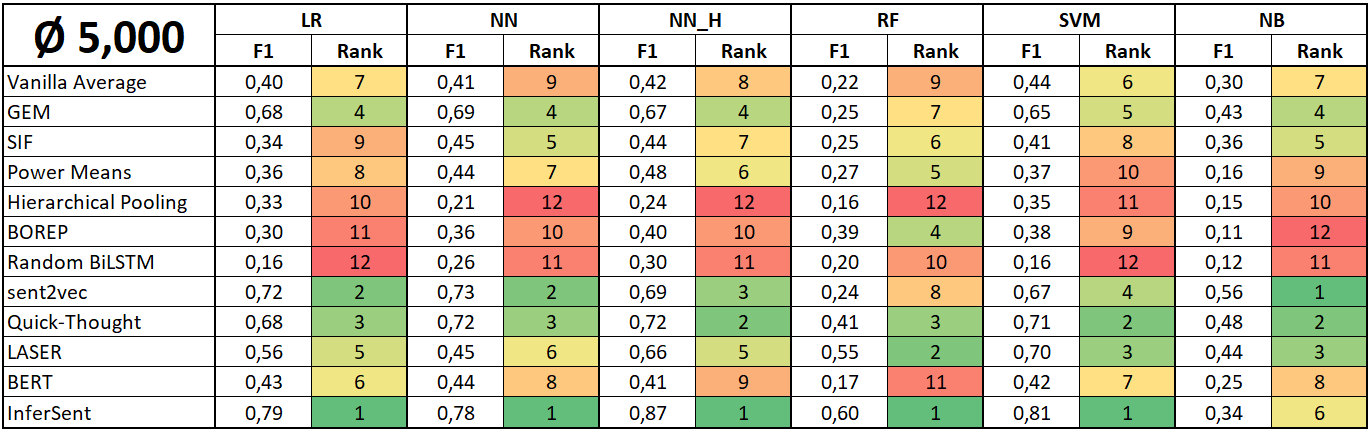
\includegraphics[scale=0.475]{images/results_wc_en_5000}
	\caption[Stability analysis results for 5k instances (\caps{WC} task, EN)]
		{Stability analysis results for 5k instances (\caps{WC} task, EN).}
\end{table}

\begin{table}[H]
	\centering
	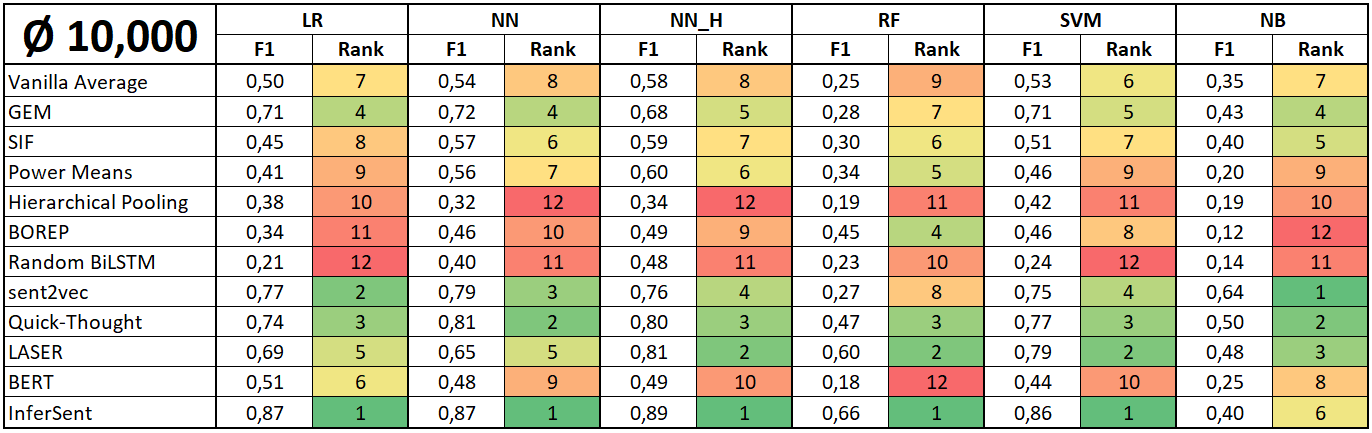
\includegraphics[scale=0.475]{images/results_wc_en_10000}
	\caption[Stability analysis results for 10k instances (\caps{WC} task, EN)]
		{Stability analysis results for 10k instances (\caps{WC} task, EN).}
\end{table}

\begin{table}[H]
	\centering
	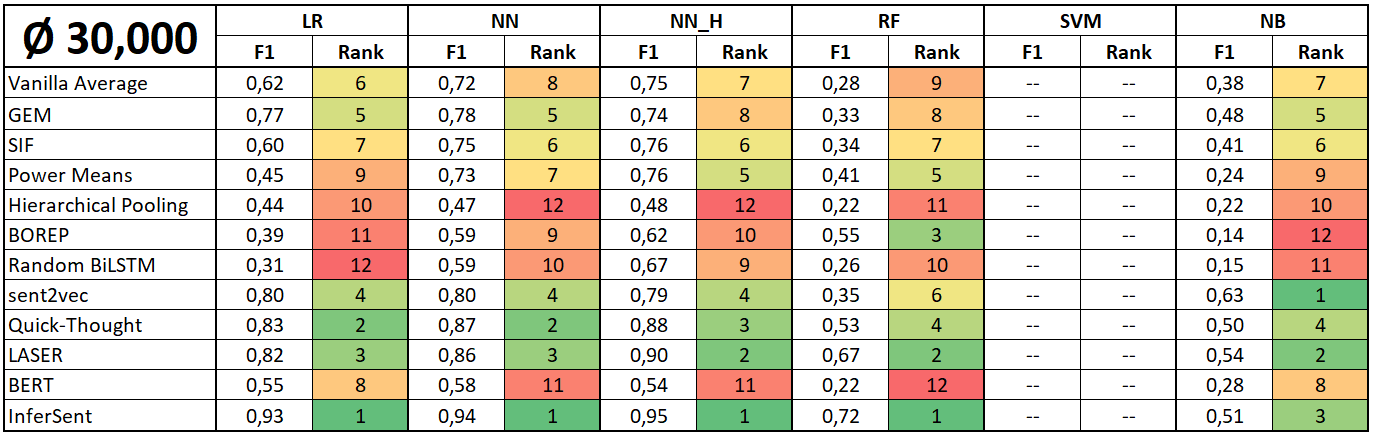
\includegraphics[scale=0.475]{images/results_wc_en_30000}
	\caption[Stability analysis results for 30k instances (\caps{WC} task, EN)]
		{Stability analysis results for 30k instances (\caps{WC} task, EN).}
\end{table}

\begin{table}[H]
	\centering
	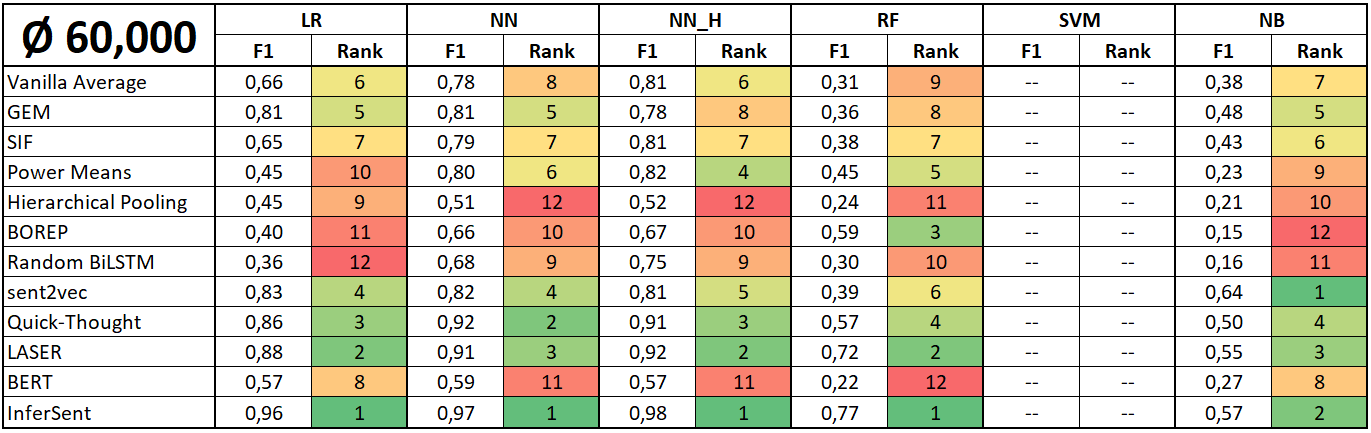
\includegraphics[scale=0.475]{images/results_wc_en_60000}
	\caption[Stability analysis results for 60k instances (\caps{WC} task, EN)]
		{Stability analysis results for 60k instances (\caps{WC} task, EN).}
\end{table}

\begin{figure}[H]
	\centering
	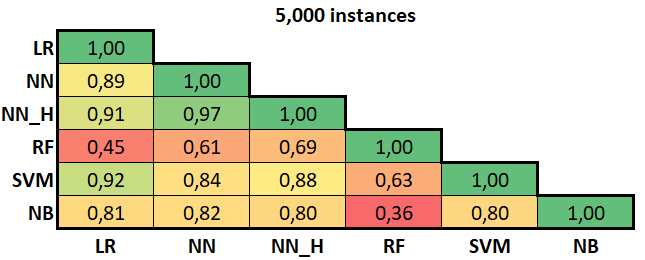
\includegraphics[scale=0.5]{images/corr_wc_en_5000}
	\caption[Classifier correlations with 5k instances (\caps{WC} task, EN)]
		{Classifier correlations with 5k instances (\caps{WC} task, EN).}
\end{figure}

\begin{figure}[H]
	\centering
	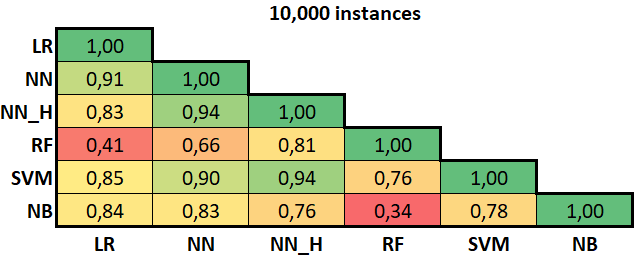
\includegraphics[scale=0.5]{images/corr_wc_en_10000}
	\caption[Classifier correlations with 10k instances (\caps{WC} task, EN)]
		{Classifier correlations with 10k instances (\caps{WC} task, EN).}
\end{figure}

\begin{figure}[H]
	\centering
	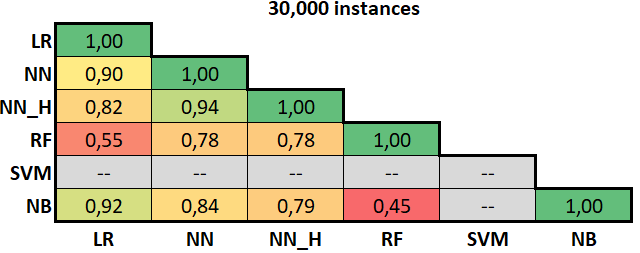
\includegraphics[scale=0.5]{images/corr_wc_en_30000}
	\caption[Classifier correlations with 30k instances (\caps{WC} task, EN)]
		{Classifier correlations with 30k instances (\caps{WC} task, EN).}
\end{figure}

\begin{figure}[H]
	\centering
	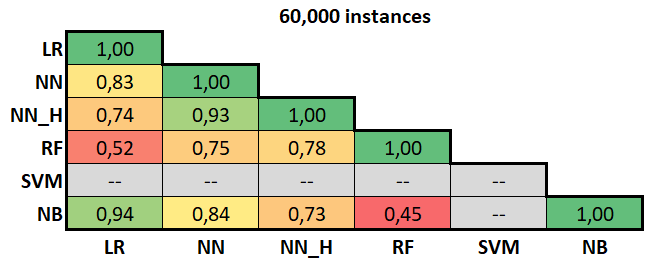
\includegraphics[scale=0.5]{images/corr_wc_en_60000}
	\caption[Classifier correlations with 60k instances (\caps{WC} task, EN)]
		{Classifier correlations with 60k instances (\caps{WC} task, EN).}
\end{figure}

% Table: Experiment results WC details deltas
\begin{table}[h]
	\centering
	\renewcommand{\arraystretch}{1.2}
	%\begin{adjustbox}{angle=90}
	\scalebox{0.9}{
	\begin{tabularx}{1.1\textwidth}{| X ? c | c | c ? c | c | c ? c | c | c ? c | c |}
		\hline
		\rowcolor{tud9c}
		\multicolumn{12}{| c |}{\textcolor{white}{\textbf{Absolute performance deltas in the \caps{WordContent} task
		(\texttt{NN\_H} classifier)}}}
		\\ \hline
		\rowcolor{tud9c!70}
													&
		\multicolumn{3}{ c ?}{
			\ding{182} $\bm{\Delta}$ \textbf{(im-)balance}} 
													&
		\multicolumn{3}{ c ?}{
			\ding{183} $\bm{\Delta}$ \textbf{(no) HP tuning}} 
													&
		\multicolumn{3}{ c ?}{
			\ding{184} $\bm{\Delta}$ \textbf{\texttt{NN} $\leftrightarrow$ \texttt{NN\_H}}}
													&
		\multicolumn{2}{ c |}{
			\ding{185} $\bm{\Delta}$ \textbf{size}}
		\\
		
		\rowcolor{tud9c!50}
		\multirow{-2}{*}{
			\cellcolor{tud9c!70}\textbf{Embedding}}	&
		\textbf{10k}		&
		\textbf{30k}		&
		\textbf{60k}		&
		\textbf{10k}		&
		\textbf{30k}		&
		\textbf{60k}		&
		\textbf{10k}		&
		\textbf{30k}		&
		\textbf{60k}		&
		\textbf{10k $\leftrightarrow$ 30k} &
		\textbf{30k $\leftrightarrow$ 60k}	
		\\ \hline\hline
		Vanilla average		& 0.21 & 0.13 & 0.09 & 0.05 & 0.01 &  0.00 & -0.04 	& -0.04 & 	-0.02 & 0.09 & 0.02
		\\ \hline
		p-Means 			& 0.20 & 0.12 & 0.09 & 0.02 & 0.00 &  0.00 & -0.03 	& -0.02 & 	-0.01 & 0.08 & 0.03
		\\ \hline
		SIF 				& 0.24 & 0.14 & 0.10 & 0.05 & 0.00 &  0.01 & -0.01 	& -0.02 & 	-0.01 & 0.07 & 0.01
		\\ \hline
		GEM 				& 0.17 & 0.12 & 0.09 & 0.03 & 0.04 &  0.04 &  0.01 	&  0.02 & 	 0.03 & 0.01 & 0.01
		\\ \hline
		hier. pooling 		& 0.29 & 0.23 & 0.22 & 0.03 & 0.01 &  0.00 & -0.04 	& -0.02 & 	-0.01 & 0.08 & 0.03
		\\ \hline
		BOREP			& 0.25 & 0.20 & 0.18 & 0.01 & 0.00 &  0.00 & -0.01	& -0.02 &	 0.00 & 0.08 & 0.03
		\\ \hline
		Random BiLSTM		& 0.23 & 0.17 & 0.14 & 0.05 & 0.00 &  0.00 & -0.08	& -0.07 &	-0.06 & 0.13 & 0.05
		\\ \hline
		InferSent 			& 0.07 & 0.03 & 0.01 & 0.01 & 0.00 &  0.00 & -0.02 	&  0.00 &  	 0.00 & 0.02 & 0.01
		\\ \hline
		Quick-Thought 		& 0.06 & 0.03 & 0.02 & 0.00 & 0.00 &  0.01 & -0.02 	&  0.00 &  	 0.00 & 0.05 & 0.02
		\\ \hline
		sent2vec 			& 0.22 & 0.20 & 0.18 & 0.01 & 0.00 &  0.00 &  0.00 	&  0.00 &  	 0.00 & 0.01 & 0.00
		\\ \hline
		BERT 			& 0.05 & 0.04 & 0.04 & 0.01 & 0.02 &  0.03 &  0.02 	&  0.03 &  	 0.02 & 0.04 & 0.03
		\\ \hline
		LASER 			& 0.09 & 0.03 & 0.02 & 0.02 & 0.01 &  0.00 & -0.08 	& -0.02 & 	-0.01 & 0.03 & 0.01
		\\ \hline
	\end{tabularx}}
	%\end{adjustbox}
	\caption[Absolute F1 performance deltas in the \caps{WC} task (\texttt{NN\_H})]
		{Absolute F1 performance deltas in the \caps{WC} task (\texttt{NN\_H}):
		\ding{182} Effect of \texttt{class balance} (positive number indicates positive effect of balanced data),
		\ding{183} Effect of \texttt{hyper-parameter tuning} (on balanced data),
		\ding{184} Effect of \texttt{classifier} (on balanced data; negative values indicate worse performance of \texttt{NN}) and
		\ding{185} effect of \texttt{size} (on balanced data sets).}
	\label{tab:wc_detail_deltas}
\end{table}

% Table: Experiment results WC Details with hp optimization
\begin{table}[h]
	\centering
	\renewcommand{\arraystretch}{1.2}
	\scalebox{0.9}{
	\begin{tabularx}{1.1\textwidth}{| X | r ? c | c | c | c ? c | c | c | c ? c | c | c | c |}
		\hline
		\rowcolor{tud9c}
		\multicolumn{14}{| c |}{\textcolor{white}{\textbf{Effect of hyper-parameter tuning in the \caps{WordContent} task
		(\texttt{NN\_H} classifier)}}}
		\\ \hline
		\rowcolor{tud9c!70}
													&
													&
		\multicolumn{4}{ c ?}{\textbf{10k}} 			&
		\multicolumn{4}{ c ?}{\textbf{30k}} 			&
		\multicolumn{4}{ c |}{\textbf{60k}}		
		\\
		
		\rowcolor{tud9c!50}
		\multirow{-2}{*}{
			\cellcolor{tud9c!70}\textbf{Embedding}}	&
		\multirow{-2}{*}{
			\cellcolor{tud9c!70}\textbf{Dim.}}			&
		\textbf{imbal.}								&
		\textbf{R}									&
		\textbf{bal.}									&
		\textbf{R}									&
		\textbf{imbal.}								&
		\textbf{R}									&
		\textbf{bal.}									&
		\textbf{R}									&
		\textbf{imbal.}								&
		\textbf{R}									&
		\textbf{bal.}									&
		\textbf{R}									
		\\ \hline\hline
%		\rowcolor{tud9c!30}
%		\multicolumn{14}{| c |}{\textbf{Neural net with hidden layer (\texttt{NN\_H}) \underl{and} hyper-parameter tuning}}
%		\\ \hline
		Vanilla average		& 300	& 0.70 & 8 	& 0.84 & 7  	& - & - & 0.89 & 7 	& - & - & 0.90 & 8 	
		\\ \hline
		p-Means			& 1,500	& 0.74 & 7 	& 0.82 & 8 	& - & - & 0.88 & 8 	& - & - & 0.91 & 6 	
		\\ \hline
		\gls{sif} 			& 300	& 0.79 & 6 	& 0.88 & 4 	& - & - & 0.90 & 5 	& - & - & 0.92 & 5 	
		\\ \hline
		\gls{gem} 			& 300 	& 0.84 & 4 	& 0.88 & 4 	& - & - & 0.90 & 5 	& - & - & 0.91 & 6 	
		\\ \hline
		hier. pooling		& 300	& 0.48 & 12 	& 0.66 & 11 	& - & - & 0.72 & 11 	& - & - & 0.74 & 11 	
		\\ \hline
		BOREP			& 4,096	& 0.53 & 11	& 0.75 & 10	& - & - & 0.82 &	 10	& - & - & 0.85 & 10
		\\ \hline
		Random BiLSTM		& 8,129	& 0.63 & 9		& 0.76 & 9		& - & - & 0.84 &	 9	& - & - & 0.89 & 9
		\\ \hline
		InferSent			& 4,096	& 0.93 & 1 	& 0.97 & 2 	& - & - & 0.98 & 2 	& - & - & 0.99 & 1 	
		\\ \hline
		Quick-Thought		& 2,400	& 0.87 & 3 	& 0.86 & 6 	& - & - & 0.91 & 4 	& - & - & 0.94 & 3 	
		\\ \hline
		sent2vec			& 700	& 0.80 & 5 	& 0.99 & 1 	& - & - & 0.99 & 1 	& - & - & 0.99 & 1 	
		\\ \hline
		BERT				& 768	& 0.55 & 10 	& 0.55 & 12 	& - & - & 0.60 & 12 	& - & - & 0.64 & 12 	
		\\ \hline
		LASER			& 1,024	& 0.90 & 2 	& 0.92 & 3 	& - & - & 0.94 & 3 	& - & - & 0.94 & 3 	
		\\ \hline
	\end{tabularx}}
	\caption[Effect of hyper-parameter tuning on the \caps{WC} probing task results (F1 scores)]
		{Effect of hyper-parameter tuning on the \caps{WC} probing task results (F1 scores). The results are
		reported for the \texttt{NN\_H} classifier.}
	\label{tab:wc_detail_hp_opt}
\end{table}

% Table: Experiment results WC details
\begin{table}[H]
	\centering
	\renewcommand{\arraystretch}{1.4}
	\scalebox{0.9}{
	\begin{tabularx}{1.1\textwidth}{| X | r ? c | c | c | c ? c | c | c | c ? c | c | c | c |}
		\hline
		\rowcolor{tud9c}
		\multicolumn{14}{| c |}{\textcolor{white}{\textbf{Effects of data set size and class balance in the
		\caps{WordContent} task}}}
		\\ \hline
		\rowcolor{tud9c!70}
													&
													&
		\multicolumn{4}{ c ?}{\textbf{10k}} 			&
		\multicolumn{4}{ c ?}{\textbf{30k}} 			&
		\multicolumn{4}{ c |}{\textbf{60k}}		
		\\
		
		\rowcolor{tud9c!50}
		\multirow{-2}{*}{
			\cellcolor{tud9c!70}\textbf{Embedding}}	&
		\multirow{-2}{*}{
			\cellcolor{tud9c!70}\textbf{Dim.}}			&
		\textbf{imbal.}								&
		\textbf{R}									&
		\textbf{bal.}									&
		\textbf{R}									&
		\textbf{imbal.}								&
		\textbf{R}									&
		\textbf{bal.}									&
		\textbf{R}									&
		\textbf{imbal.}								&
		\textbf{R}									&
		\textbf{bal.}									&
		\textbf{R}									
		\\ \hline\hline
		\rowcolor{tud9c!30}
		\multicolumn{14}{| c |}{\textbf{Neural network with hidden layer (\texttt{NN\_H})}}
		\\ \hline
		Vanilla average	& 300 	& 0.58 & 8 	& 0.79 & 8  	& 0.75 & 7 	& 0.88 & 6 	& 0.81 & 5 	& 0.90 & 7 	
		\\ \hline
		p-Means 		& 1,500 	& 0.60 & 6 	& 0.80 & 7  	& 0.76 & 5 	& 0.88 & 6 	& 0.82 & 4		& 0.91 & 5 	
		\\ \hline
		\gls{sif} 		& 300	& 0.59 & 7 	& 0.83 & 6  	& 0.76 & 5 	& 0.90 & 5 	& 0.81 & 5		& 0.91 & 5	
		\\ \hline
		\gls{gem} 		& 300 	& 0.68 & 5		& 0.85 & 5 	& 0.74 & 8 	& 0.86 & 8 	& 0.78 & 8		& 0.87 & 9 	
		\\ \hline
		hier. pooling	& 300	& 0.34 & 12 	& 0.63 & 11 	& 0.48 & 12 	& 0.71 & 11	& 0.52 & 12	& 0.74 & 11
		\\ \hline
		BOREP 		& 4,096	& 0.49 & 9		& 0.74 & 9		& 0.62 & 10	 & 0.82 & 10	& 0.67 & 10	& 0.85 & 10
		\\ \hline
		Random BiLSTM & 8,129	& 0.48 & 11	& 0.71 & 10	& 0.67 & 9		& 0.84 & 9		& 0.75 & 9		& 0.89 & 8
		\\ \hline
		InferSent		& 4,096	& 0.89 & 1		& 0.96 & 2		& 0.95 & 1 	& 0.98 & 2		& 0.98 & 1		& 0.99 & 1 	
		\\ \hline
		Quick-Thought	& 2,400	& 0.80 & 3		& 0.86 & 4		& 0.88 & 3 	& 0.91 & 4		& 0.91 & 3		& 0.93 & 4 	
		\\ \hline
		sent2vec		& 700	& 0.76 & 4 	& 0.98 & 1 	& 0.79 & 4 	& 0.99 & 1 	& 0.81 & 5		& 0.99 & 1	
		\\ \hline
		BERT			& 768	& 0.49 & 9 	& 0.54 & 12 	& 0.54 & 11 	& 0.58 & 12 	& 0.57 & 11	& 0.61 & 12	
		\\ \hline
		LASER		& 1,024	& 0.81 & 2 	& 0.90 & 3		& 0.90 & 2		& 0.93 & 3 	& 0.92 & 2		& 0.94 & 3	
		\\ \hline\hline
		\rowcolor{tud9c!30}
		\multicolumn{14}{| c |}{\textbf{Neural net without hidden layer (\texttt{NN})}}
		\\ \hline
		Vanilla average 		& 300 	& 0.54 & 8 	& 0.75 & 8 	& 0.72 & 8 	& 0.84 & 8		& 0.78 & 8 	& 0.88 & 8 	
		\\ \hline
		p-Means 			& 1,500 	& 0.56 & 7 	& 0.77 & 7		& 0.73 & 7 	& 0.86 & 7 	& 0.80 & 6 	& 0.90 & 5	
		\\ \hline
		\gls{sif} 			& 300	& 0.57 & 6		& 0.82 & 5		& 0.75 & 6 	& 0.88 & 5		& 0.79 & 7 	& 0.90 & 5	
		\\ \hline
		\gls{gem} 			& 300 	& 0.72 & 4		& 0.86 & 3 	& 0.78 & 5 	& 0.88 & 5		& 0.81 & 5 	& 0.90 & 5	
		\\ \hline
		hier. pooling		& 300	& 0.32 & 12	& 0.59 & 11	& 0.47 & 12	& 0.69 & 11	& 0.51 & 12 	& 0.73 & 11	
		\\ \hline
		BOREP 			& 4,096	& 0.46 & 10	& 0.73 & 9		& 0.59 & 9	 	& 0.80 & 9		& 0.66 & 10	& 0.85 & 9
		\\ \hline
		Random BiLSTM 	& 8,129	& 0.40 & 11	& 0.63 & 10	& 0.59 & 9		& 0.77 & 10	& 0.68 & 9		& 0.83 & 10
		\\ \hline
		InferSent			& 4,096	& 0.87 & 1		& 0.94 & 2		& 0.94 & 1 	& 0.98 & 2		& 0.97 & 1 	& 0.99 & 1 	
		\\ \hline
		Quick-Thought		& 2,400	& 0.81 & 2		& 0.84 & 4		& 0.87 & 2 	& 0.91 & 3 	& 0.92 & 2 	& 0.93 & 3
		\\ \hline
		sent2vec			& 700	& 0.79 & 3		& 0.98 & 1 	& 0.80 & 4 	& 0.99 & 1		& 0.82 & 4 	& 0.99 & 1	
		\\ \hline
		BERT				& 768	& 0.48 & 9		& 0.56 & 12	& 0.58 & 11 	& 0.61 & 12	& 0.59 & 11 	& 0.63 & 12	
		\\ \hline
		LASER			& 1,024	& 0.65 & 5		& 0.82 & 5		& 0.86 & 3		& 0.91 & 3		& 0.91 & 3		& 0.93 & 3	
		\\ \hline
	\end{tabularx}}
	\caption[Effects of class (im-)balance as well as data set size on the \caps{WC} probing task results (F1 scores)]
		{Effects of class (im-)balance as well as data set size on the results for the \caps{WC} probing task (F1 scores). The results are
		reported for the \texttt{NN\_H} classifier (top) as well as for the \texttt{NN} classifier (bottom).}
	\label{tab:wc_detail}
\end{table}

\newpage

% Georgian
% -----------------------------------------------------------------------------------------------------------------------------------------------------
\subsection{Georgian}

\begin{table}[H]
	\centering
	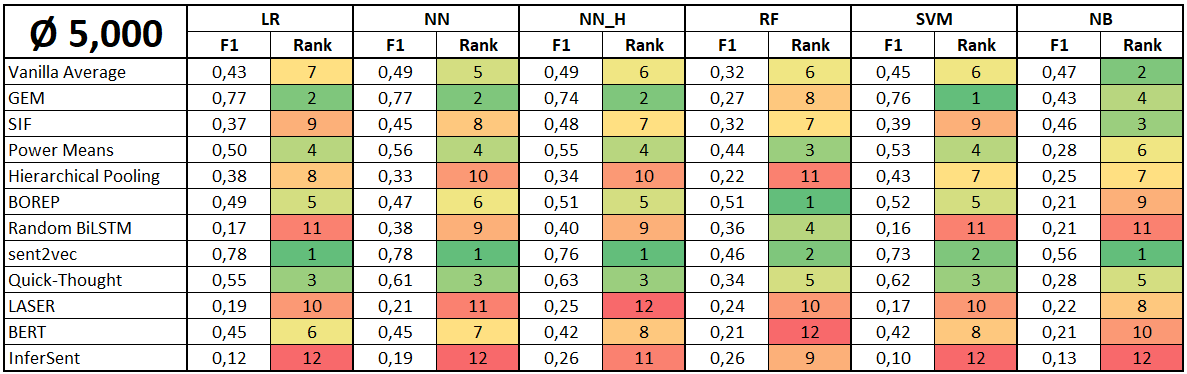
\includegraphics[scale=0.55]{images/results_wc_ka_5000}
	\caption[Stability analysis results for 5k instances (\caps{WC} task, KA)]
		{Stability analysis results for 5k instances (\caps{WC} task, KA).}
\end{table}

\begin{table}[H]
	\centering
	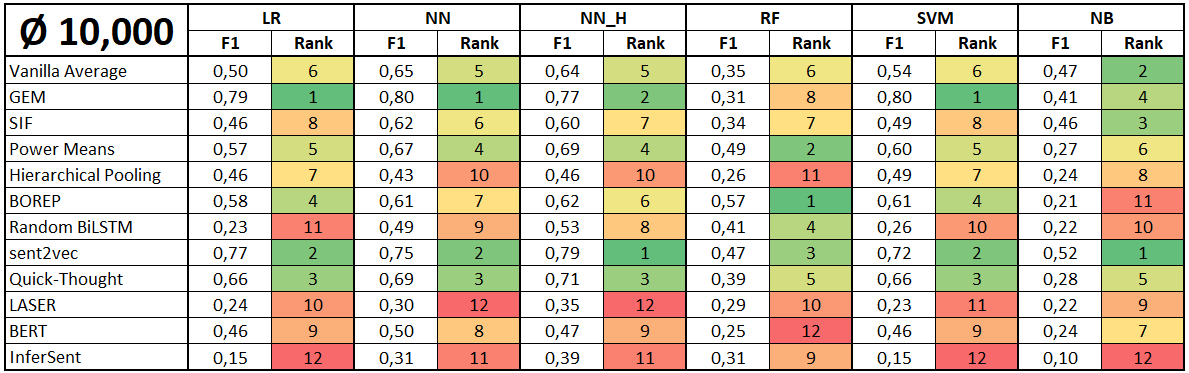
\includegraphics[scale=0.55]{images/results_wc_ka_10000}
	\caption[Stability analysis results for 10k instances (\caps{WC} task, KA)]
		{Stability analysis results for 10k instances (\caps{WC} task, KA).}
\end{table}

\begin{table}[H]
	\centering
	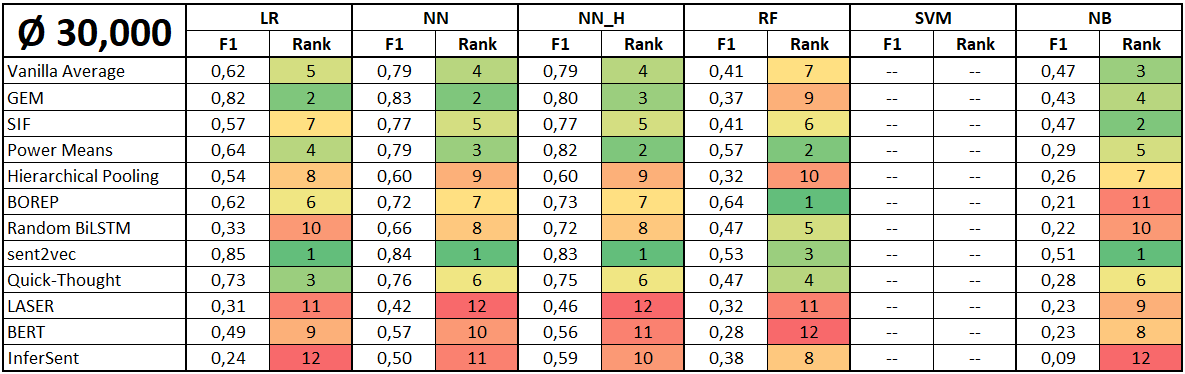
\includegraphics[scale=0.55]{images/results_wc_ka_30000}
	\caption[Stability analysis results for 30k instances (\caps{WC} task, KA)]
		{Stability analysis results for 30k instances (\caps{WC} task, KA).}
\end{table}

\begin{table}[H]
	\centering
	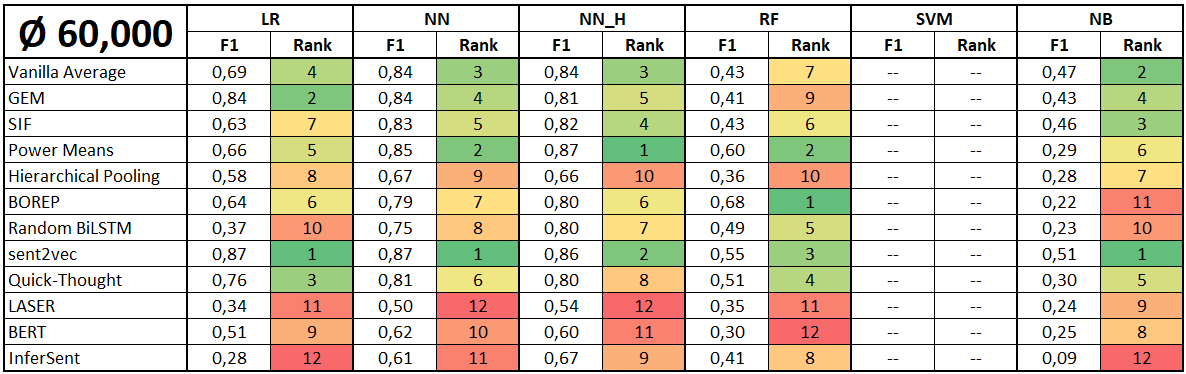
\includegraphics[scale=0.55]{images/results_wc_ka_60000}
	\caption[Stability analysis results for 60k instances (\caps{WC} task, KA)]
		{Stability analysis results for 60k instances (\caps{WC} task, KA).}
\end{table}

\begin{figure}[H]
	\centering
	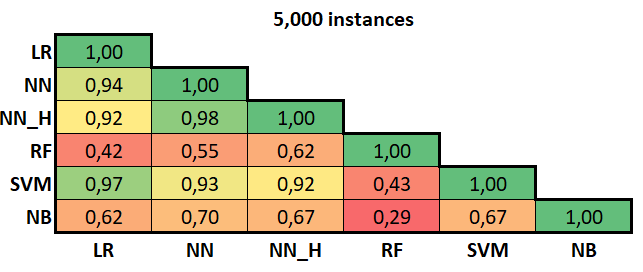
\includegraphics[scale=0.5]{images/corr_wc_ka_5000}
	\caption[Classifier correlations with 5k instances (\caps{WC} task, KA)]
		{Classifier correlations with 5k instances (\caps{WC} task, KA).}
\end{figure}

\begin{figure}[H]
	\centering
	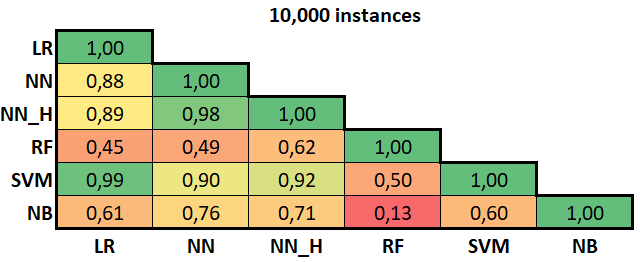
\includegraphics[scale=0.5]{images/corr_wc_ka_10000}
	\caption[Classifier correlations with 10k instances (\caps{WC} task, KA)]
		{Classifier correlations with 10k instances (\caps{WC} task, KA).}
\end{figure}

\begin{figure}[H]
	\centering
	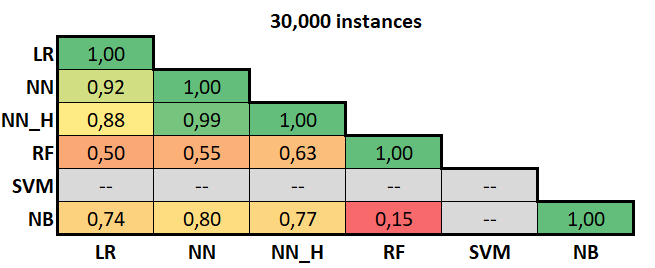
\includegraphics[scale=0.5]{images/corr_wc_ka_30000}
	\caption[Classifier correlations with 30k instances (\caps{WC} task, KA)]
		{Classifier correlations with 30k instances (\caps{WC} task, KA).}
\end{figure}

\begin{figure}[H]
	\centering
	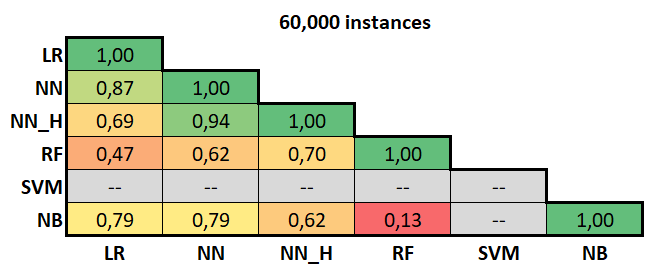
\includegraphics[scale=0.5]{images/corr_wc_ka_60000}
	\caption[Classifier correlations with 60k instances (\caps{WC} task, KA)]
		{Classifier correlations with 60k instances (\caps{WC} task, KA).}
\end{figure}